% Describe RCPS Testbed & Testing Platform
% Describe evaluation metrics
% Describe testing scenarios and use cases
\chapter{Experimental Evaluation}
\label{chapter:evaluation}

Experimentally validating our timing analysis results is an important and necessary requirement. In order to obtain any level of confidence in our CPN-based work, the system design model needs to be completed implemented, and deployed on the target hardware platform. We have constructed a testbed \cite{kumarTestbed} to simulate and analyze resilient cyber-physical systems consisting of 32 Beaglebone Black development boards \cite{BBB}. We have chosen the light-weight ROS \cite{ROS} middleware layer and implemented our ROSMOD Component model \cite{kumarROSMOD} on top of it. This component model provides the same execution semantics and interaction patterns as our DREMS component model \cite{ISIS_F6_ISORC:13}. Our goal with this work is to (1) establish a set of distributed component-based applications, (2) translate this design model to our CPN analysis model, (3) deploy these applications on our testbed and accurately measure operation execution times, and finally (4) perform state space analysis on the generated CPN model to check for conservative results, compared against the real system execution.

\subsection{Challenges}

Experimental validation requires that online measurements of the real-time system match with the timing analysis results in a way that the timing analysis results are always close but conservative. If the timing analysis results predict a deadline violation, this does not necessarily mean that the real system will violate deadlines but if the timing analysis and verification guarantees a lack of deadline violations, then the real system should follow this prediction. One of the biggest assumptions in our CPN work is the knowledge of worst-case execution times of the individual steps in the component operations. There are various ways to obtain the WCET values for individual operational steps but the easiest approach is to execute the design into our testbed and make accurate measurements.

WCET of component operational steps needs to be measured by having the component operation execute at real-time priority with no other component threads intervening this process. This measurement gives us a \emph{pure execution time} of the code block. The process must be repeated for all component operations to obtain meaningful worst-case estimates that are tailored to the target platform. Obtaining the WCET values by this method is not only more realistic but also an accurate representation of the target system. Once these individual numbers are obtained, the values are plugged into the CPN through our business-logic models. Ideally, the CPN model, consisting of a composition of component operation models, when analyzed, produces results that closely resemble a real-system deployment of the component assembly. Such results would validate the modeling accuracy and the analysis results.

Distributed CPS are hard to develop hardware/software for; because the software is coupled with the hardware and the physical system, software testing and deployment may be difficult - a problem only exacerbated by distributing the system.  These types of systems must be tested for performance assurances, reliability, and fail-safety.  Examples of these systems include UAV/UUV systems, fractionated satellite clusters, and networks of autonomous vehicles, all of which require strict guarantees about not only the performance of the system, but also the reliability of the system.  Because of the need for such strict design-time guarantees, many traditional techniques for software testing cannot be used.  Cloud-based software testing may not accurately reflect the performance of the software, since many of these systems use specialized embedded computers, and furthermore does not provide the capability to easily integrate a system simulation into the software testing loop.  For such systems, a closed-loop simulation testbed is necessary which can fully emulate the deployed system, including the physical characteristics of the nodes, the network characteristics of the systems, and the sensors and actuators used by the systems.

Emerging industry standards and collaborations are progressing towards component-based system development and reuse, \emph{e.g.} AUTOSAR~\cite{autosar} in the automotive industry.  As these systems are becoming increasingly more reliant on collections of software components which must interact, they enable more advanced features, such as better safety or performance, but as a consequence require more thorough integration testing.  Comprehensive full systems integration is required for system analysis and deployment, and the development of relevant testing system architectures enables expedited iterative integration.  Developing these systems iteratively, by prototyping individual components and composing them can be expensive and time consuming, so tools and techniques are needed to expedite this process.  Our testbed architecture was developed to help address these issues and decrease the turn-around time for integration testing of distributed, resilient CPS.  

Examples of such systems which can be prototyped and tested using this architecture are (1) autonomous cars, (2) controllers for continuous and discrete manufacturing plants, and (3) UAV swarms.  Each of these systems is characterized as a distributed CPS in which embedded controllers are networked to collectively control a system through cooperation.  Each subsystem or embedded computer senses and controls a specific aspect of the overall system and cooperates to achieve the overall system goal.  For instance, the autonomous car's subsystems of global navigation, pedestrian detection, lane detection, engine control, brake control, and steering control all must communicate and cooperate together to achieve full car autonomy.  The control algorithms for each of these subsystems must be tested with their sensors and actuators but also must be tested together with the rest of the systems.  It is these types of cooperating embedded controllers which are a distinguishing feature of distributed CPS.  Integration testing for these distributed CPS can be quickly and easily accomplished using hardware-in-the-loop simulation, but must accurately represent the real physical system, hardware, software, and network. 

In scenarios like the automotive networked CPS, one of the main challenges with system testing is the discord between the standardized networking protocols and communication methods e.g. CAN bus, and the manufacturer-specific implementations of these methods. It is difficult to obtain public access to the implementation details for such interaction patterns and therefore pure simulation of the communication protocols using event-simulation tools  is not sufficient in validating resilient application performance. The comprehensive testing for such safety-critical systems require \emph{replicating the CPS} by using a testing infrastructure that provides similar hardware and executes the exact embedded control code that would execute on the final system. 

% Section on our RCPS Testbed
\section{Resilient Cyber-Physical Systems (RCPS) Testbed}

\subsection{Architecture}

Cyber-Physical Systems require design-time testing and analysis before deployment. Several CPS scenarios require strict safety certification due to the mission-critical nature of the operation, e.g. flight
control and automation. It is often times impossible to test control algorithms, fault tolerance procedures etc. on the real system due to both cost and hardware accessibility issues. To counter these issues, there are two principle methods in which a CPS can be tested and analyzed: (1) Construct a complete model of the CPS in a simulation environment e.g. Simulink \cite{Simulink} and simulate the system
while accounting for run-time scenarios, (2) Establish a testing environment that can closely resemble the real CPS in both hardware and software. The problem with simulations is that it is hard to
establish the network topology, emulate the application network and base processing power while running a physics simulation in the loop. Our RCPS architecture implements the latter alternative, as shown in Figure \ref{fig:architecture}. We believe that a generic testing environment that uses embedded boards, programmable network switches and physics simulation machines like this, is the most suitable solution to emulate real CPS deployments.

\begin{figure}[h]
    \centering
    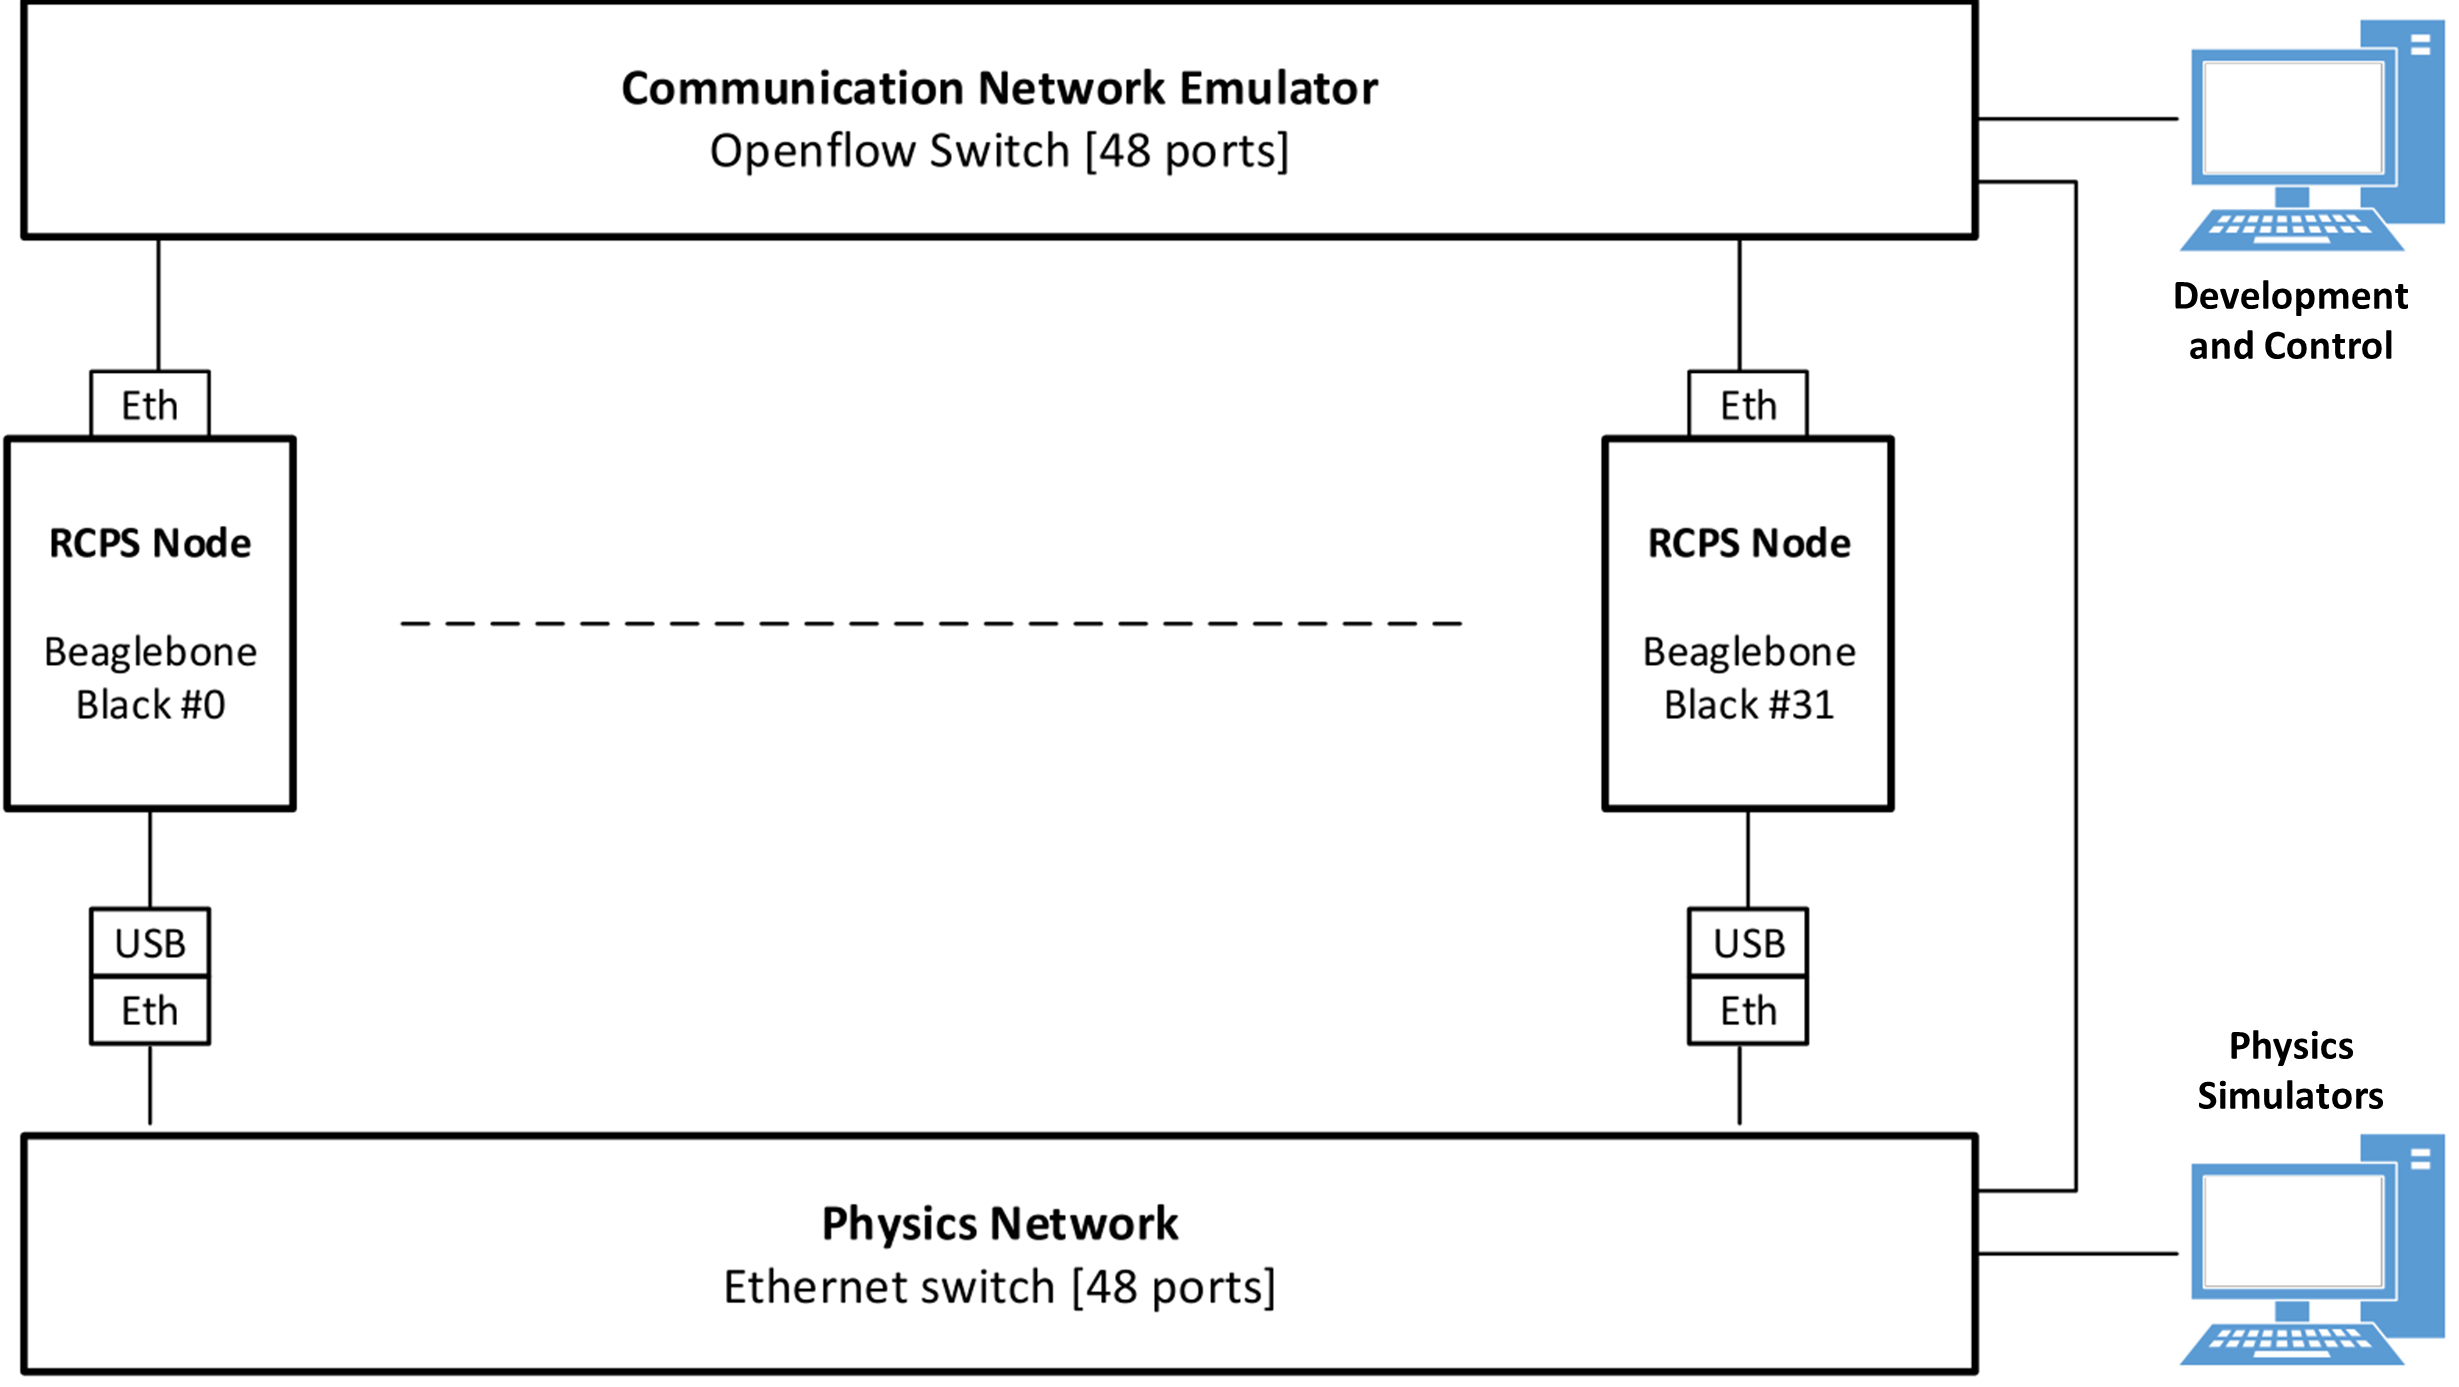
\includegraphics[width=\textwidth]{rcps-architecture.png}
    \caption{Testbed Architecture}
    \label{fig:architecture}
\end{figure}

The testbed consists of 32 \emph{RCPS nodes}, each of which is a Beaglebone Black (BBB) \cite{BBB} development board running Linux, as shown in Figure \ref{fig:boards}. We execute a full software stack including a ROS-based middleware, called ROSMOD \cite{kumarROSMOD} and the DREMS component model. For the subset of CPS we are interested in, the behavior of the CPS can be much more precisely emulated with these boards compared to running the applications inside of a standalone simulation. For example, NASA's CubeSat Launch Initiative (CSLI) \cite{CubeSat} provides opportunities for nanosatellites to be deployed into space for research. CubeSats are small (4-inch long) satellites running low-power embedded boards and being prepared for interplanetary missions \cite{CubeSat_Mars} to Mars. A distributed set of CubeSats can be easily tested with this architecture if it can be integrated with a high-fidelity space flight simulator.  

\begin{figure}[h]
    \centering
    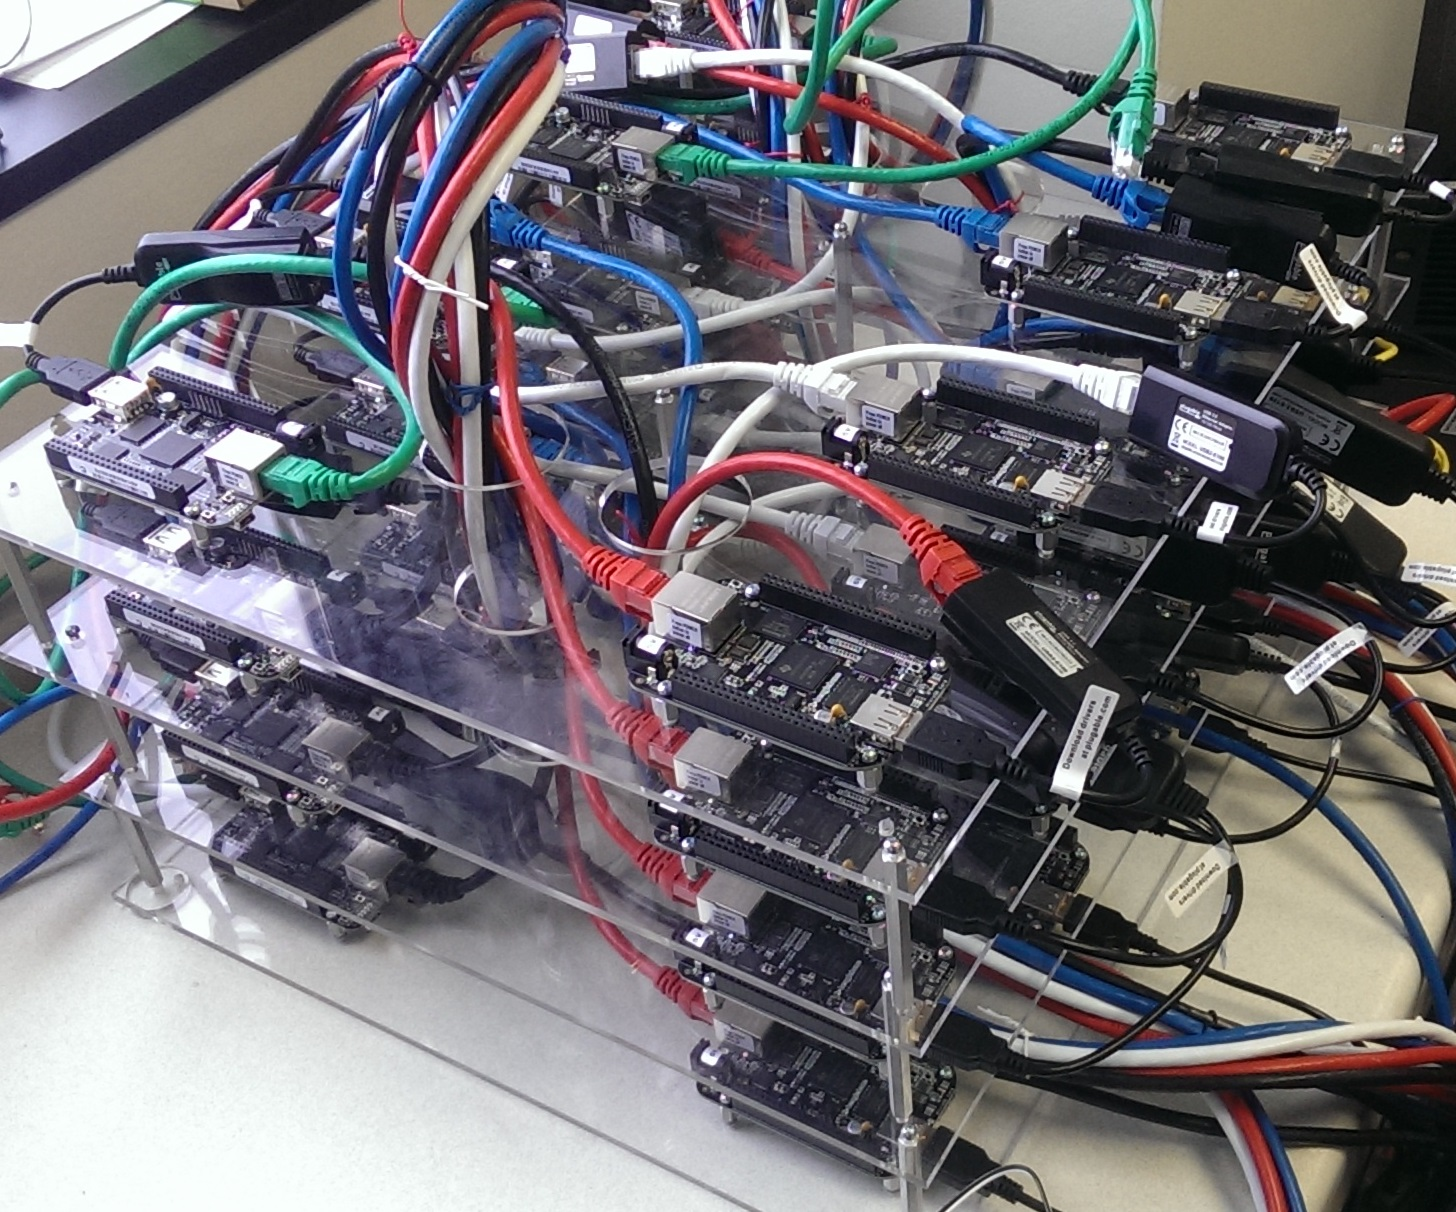
\includegraphics[width=0.9\textwidth]{bbb}
    \caption{Beaglebone Black Boards - Custom Mounting}
    \label{fig:boards}
\end{figure}

The Gigabit Ethernet port of each BBB is connected to a \emph{Communication Network} switch. This is a programmable OpenFlow \cite{openflow} switch, allowing users to program the flowtable of the switch to control the routes that packets follow and completely configure the full network and subnets required for their emulated deployment.  Furthermore, the configurability of the communications network enables per-link or per-flow bandwidth throttling, enabling precise network emulation.  The primary \emph{Development and Control} machine, running our software development tools, communicates with the BBBs using this network. After software applications are deployed on this testbed, the characteristics of the real CPS network can be enforced on the application network traffic. Therefore, this network emulates the physical network which a distributed CPS would experience on deployment.

Each RCPS node is also connected to a \emph{Physics Network} using a 10/100 USB-to-Ethernet adapter, since the BBBs only have one gigabit ethernet port. This network is connected to a \emph{Physics Simulation Machine} running Cyber-Physical Systems simulations. This network provides the infrastructure necessary to emulate CPS sensing and actuation in the loop, allowing application software to periodically receive sensor data and open interfaces to output actuator commands to the simulation.

The Physics Simulation Machine closes the interaction loop for the testbed nodes, allowing the physical dynamics of the RCPS nodes to be simulated in the environment in which it would be deployed, \emph{e.g.} satellites' orbital mechanics and interactions can be simulated for a satellite cluster in low Earth orbit (LEO). 

\subsection{Design and Construction}

The RCPS testbed was designed and constructed to be as self-contained as possible, while allowing for extensibility and modularity. The 32 BBB development boards were arranged on 4 laser-cut acrylic plates, with 8 boards on each plate, as shown in Figure \ref{fig:boards}. Holes on each plate route network and power supply cables from/to each board. With the communication network switch on top of these boards and the physics network switch on the bottom, the ensemble takes a total of 8U (rack units) of space. The primary power supply is an off-the-shelf 300 W power supply with custom cabling to fan-out power to all 32 boards in an efficient manner.  By configuring the testbed in this self-contained way, we can easily maintain it, monitor it, and move it should the need arise.  

\begin{figure}[h]
    \centering
    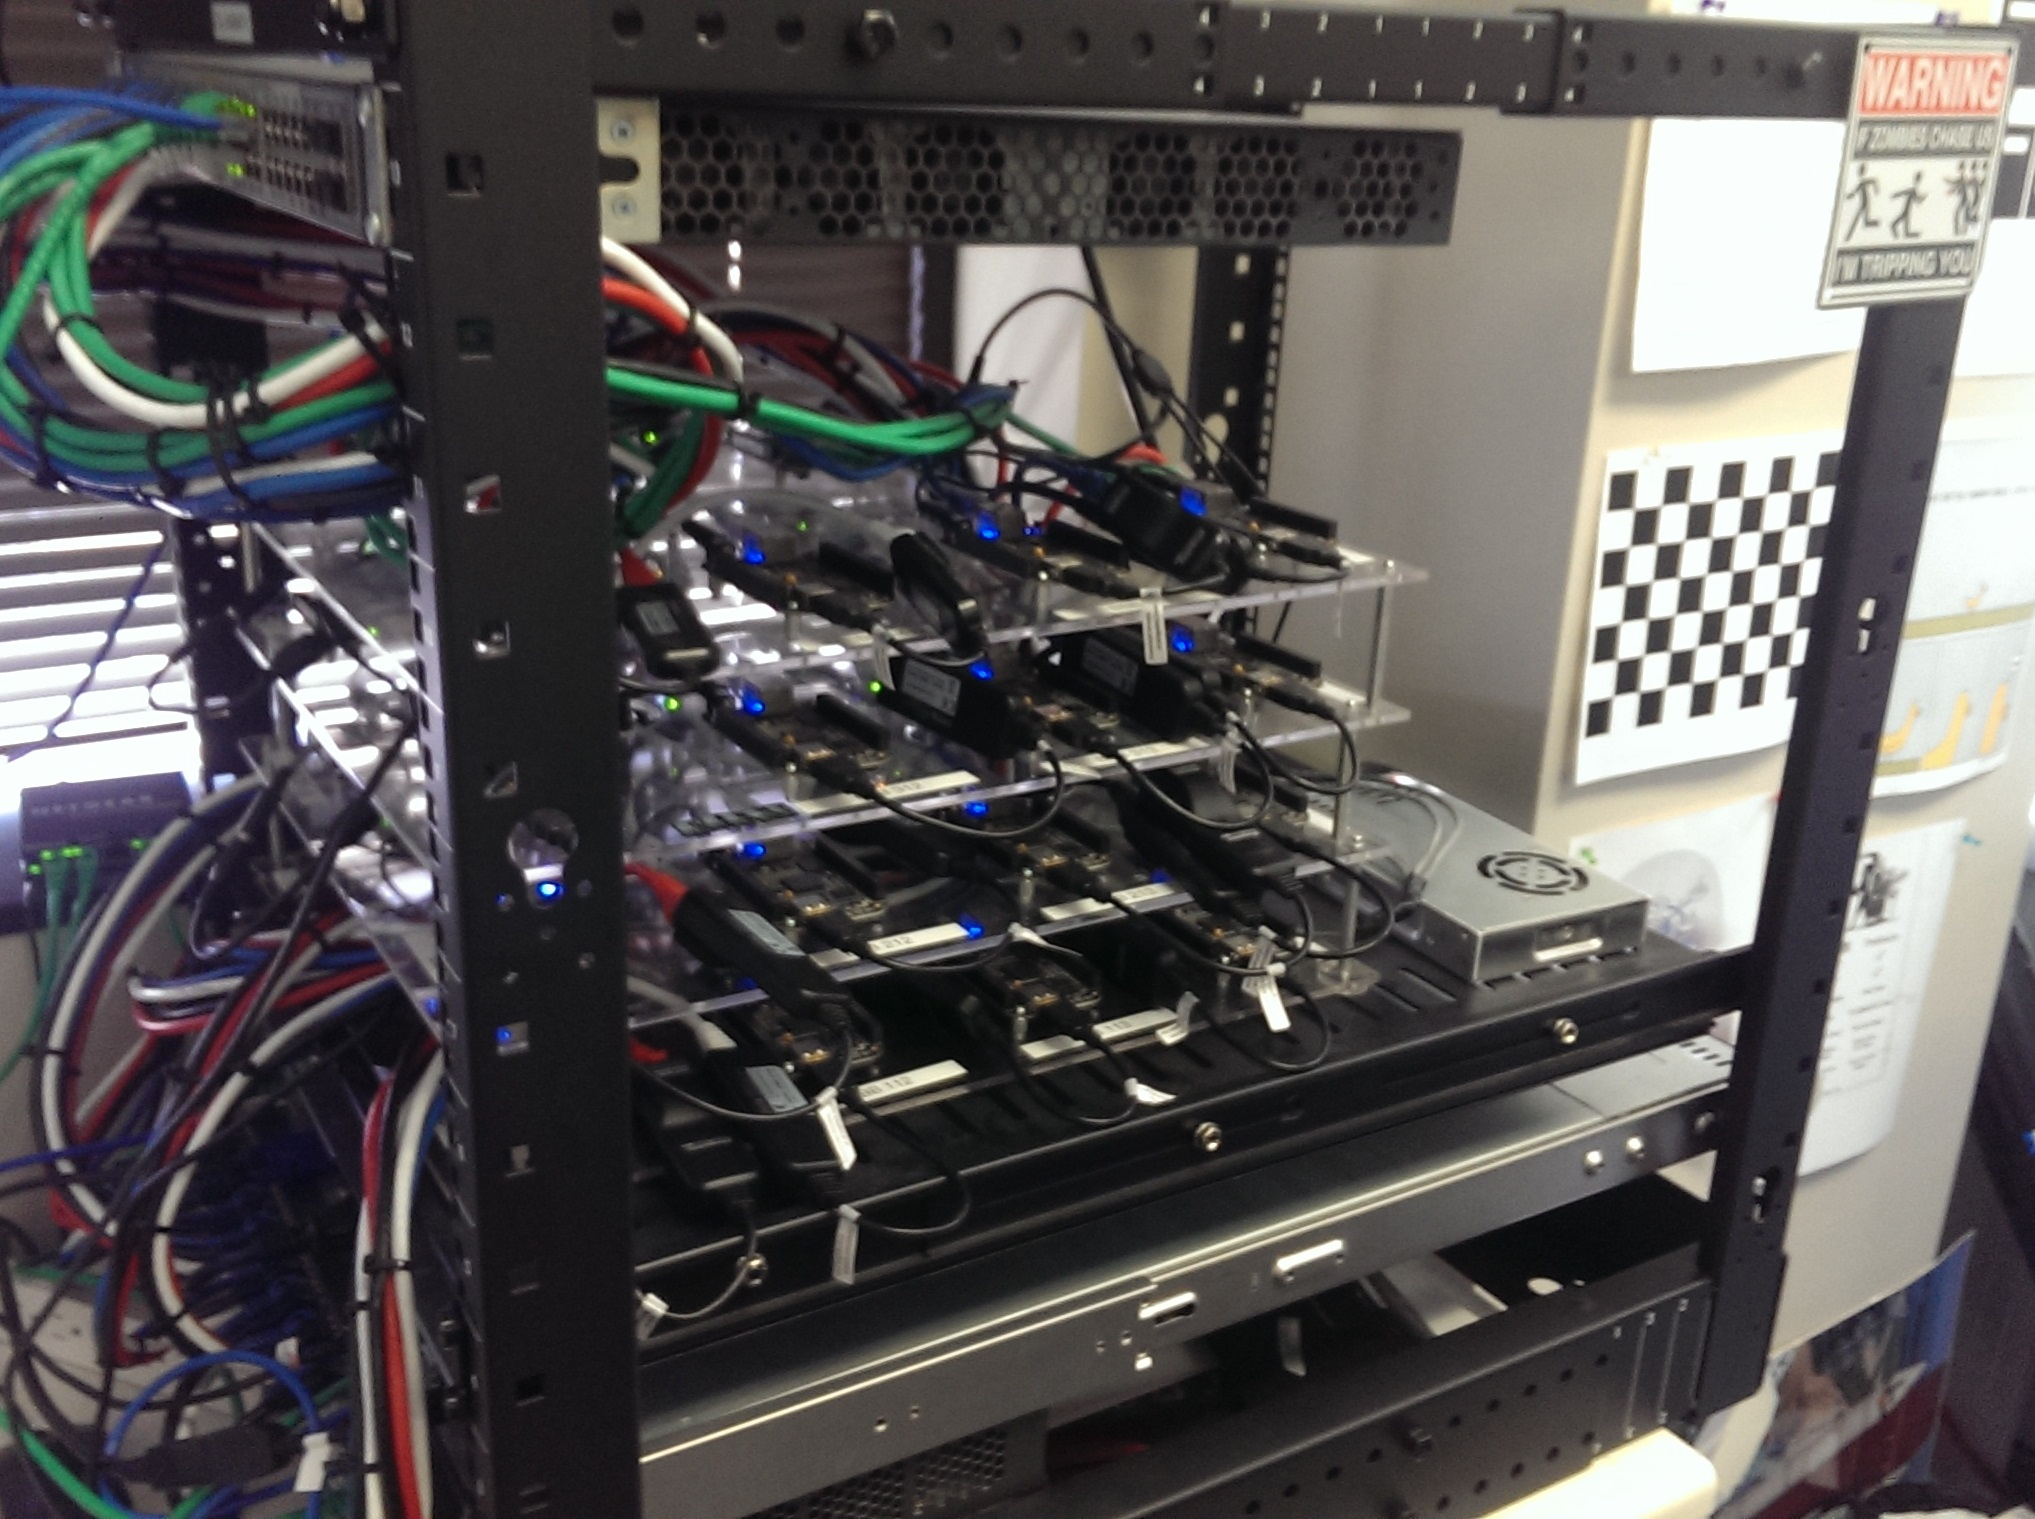
\includegraphics[width=\textwidth]{testbed}
    \caption{Constructed Testbed}
    \label{fig:testbed}
\end{figure}

Using a 13U server cabinet and standard mounting equipment, the network switches and simulation machines are mounted on either side of the development boards. Figure \ref{fig:testbed} shows the fully mounted testbed. The cabinet supports mountable base wheels which makes this setup easily portable. 

\section{ROSMOD Software Infrastructure}

The software infrastructure includes our model-driven toolsuite and DREMS-style component model called ROSMOD \cite{kumarROSMOD}, the Robot Operating System middleware \cite{ROS}, and component-based software applications developed for ROSMOD. The applications are cross-compiled for Beaglebone Black and the relevant processes are started at real-time priority with \emph{SCHED\_RR} linux real-time process scheduling using our ROSMOD deployment framework (Figure \ref{fig:rosmod_deployment}).

\subsubsection{ROSMOD Modeling Language}

ROSMOD Projects are built using the ROSMOD Modeling Language. With this language, ROS users can create models of ROS workspaces, hardware topologies, deployment plans and more. The tool suite provides a Graphical User Interface to build these models but the state and configuration properties of the project are saved in a set of text files (models) that follow a strict set of grammatical rules, written using Antlr 4 \cite{ANTLR_BOOK}. Figure \ref{fig:ROSMOD_Project} shows the metamodel of the textual modeling language as a UML \cite{UML} class diagram.

\begin{figure}[h]
    \centering
    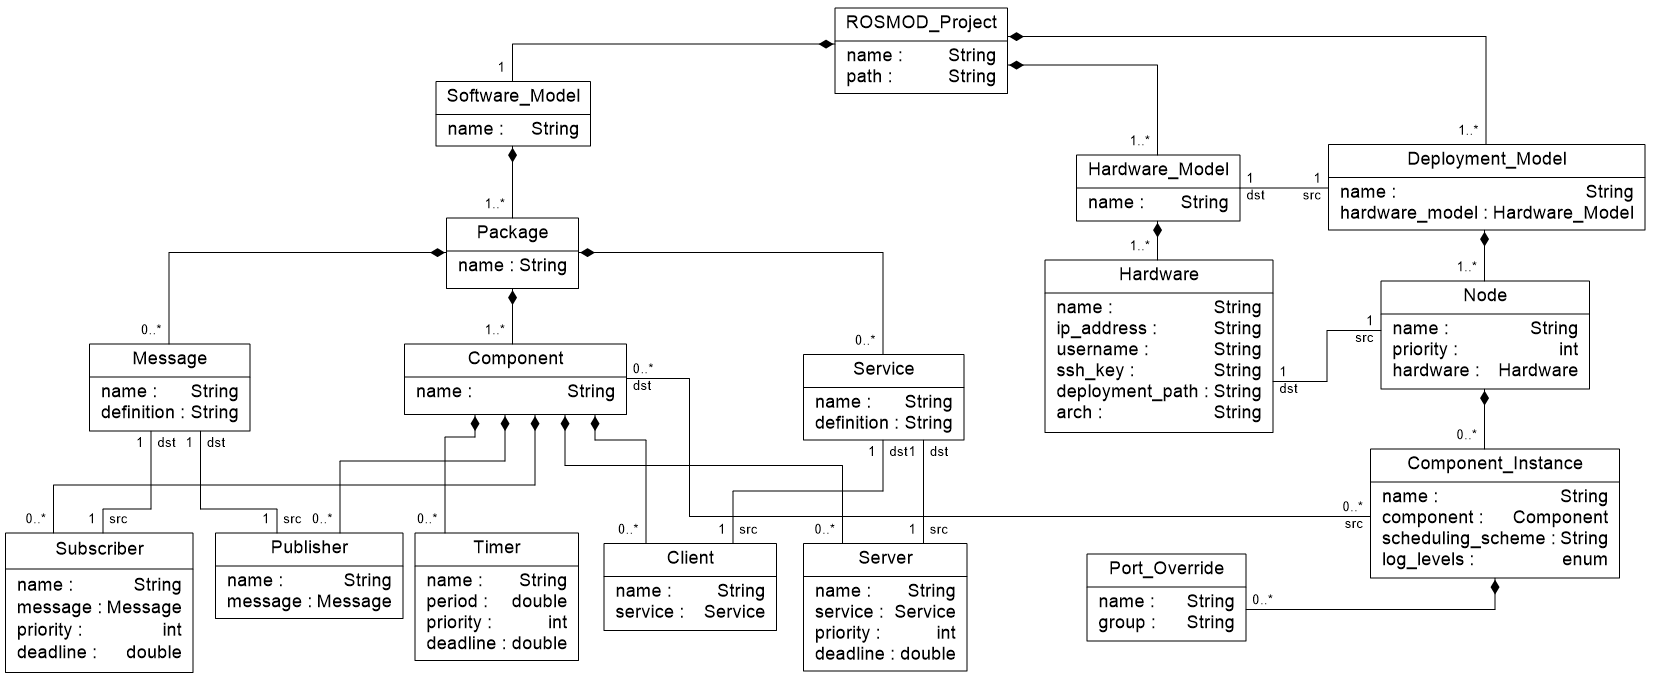
\includegraphics[width=\textwidth]{ROSMOD_Project}
    \caption{ROSMOD Project}
    \label{fig:ROSMOD_Project}
\end{figure}

ROS workspaces are high-level containers for source code which may contain one or more ROS packages.  ROS packages are containers which may include (1) one or more ROS message definitions for asynchronous publish/subscribe, (2) one or more ROS service definitions for synchronous RMI, and (3) one or more ROS Nodes, which are processes that can communicate with each other using predefined ROS messages or ROS services.  In this way a ROS package can be thought of as an application, and a ROS node is a process in that application.

\emph{The ROSMOD Software model} represents a ROS workspace. Each model consists of one or more ROS packages. Each ROS package contains definitions to (1) messages, (2) services and (3) components. The component assembly is derived from the interacting component ports. Ports that are associated with callbacks e.g. subscribers, contain both a \emph{priority} and a \emph{deadline} property to facilitate the scheduling schemes in the component model.

\emph{Hardware models} completely describe the hardware architecture of the system. Here, the user describes the different hardware hosts available for deployment, including their properties such as IP address, username and SSH keys.  These properties allow the user to directly map executables to hardware in a specified network and allow the deployment infrastructure to manage all remote operations and help ensure security between applications.  Deployment models refer to such predefined hardware models when mapping processes to hardware devices. Current work aims to improve on this hardware model by adding concepts for subnets, network interface controllers (NIC) and network links between hardware devices to more accurately represent the network topology.

\emph{ROSMOD Deployment models} contain the specifications for ROS nodes (executable processes). Each ROS node is ranked by a process priority and is mapped to a specific hardware device on which it will be executed. Each ROS node contains instances of software components that control its behavior. These component instances refer to specific components defined in the Software Model. At run-time, each node creates one executor thread per component instance before  beginning its interaction with the rest of the application. 

\subsubsection{Deployment Infrastructure}

The workflow for software deployment is as shown Figure \ref{fig:rosmod_deployment}. Every ROS workspace is generated with an additional \emph{node} package. This builds a generic node executable that can dynamically load libraries. Once the generators generate the ROS workspace and deployment XML files, users complete application development and build their ROS workspace. The build process generates dynamically loadable libraries, one for each component definition along with a single executable corresponding to the generic node package. The generated XML files contain metadata about about all ROS nodes modeled in the ROSMOD Deployment Model. This includes the component instances in each node and the appropriate component libraries to be loaded. Based on the XML file supplied to the node executable, the node will behave as one of the ROS nodes in the model. This allows for a reusable framework where a generic executable (1) loads an XML file, (2) identifies the component instances in the node, (3) finds the necessary component libraries to load and (4) spawns the executor threads bound to each component. 

\begin{figure}[h]
    \centering
    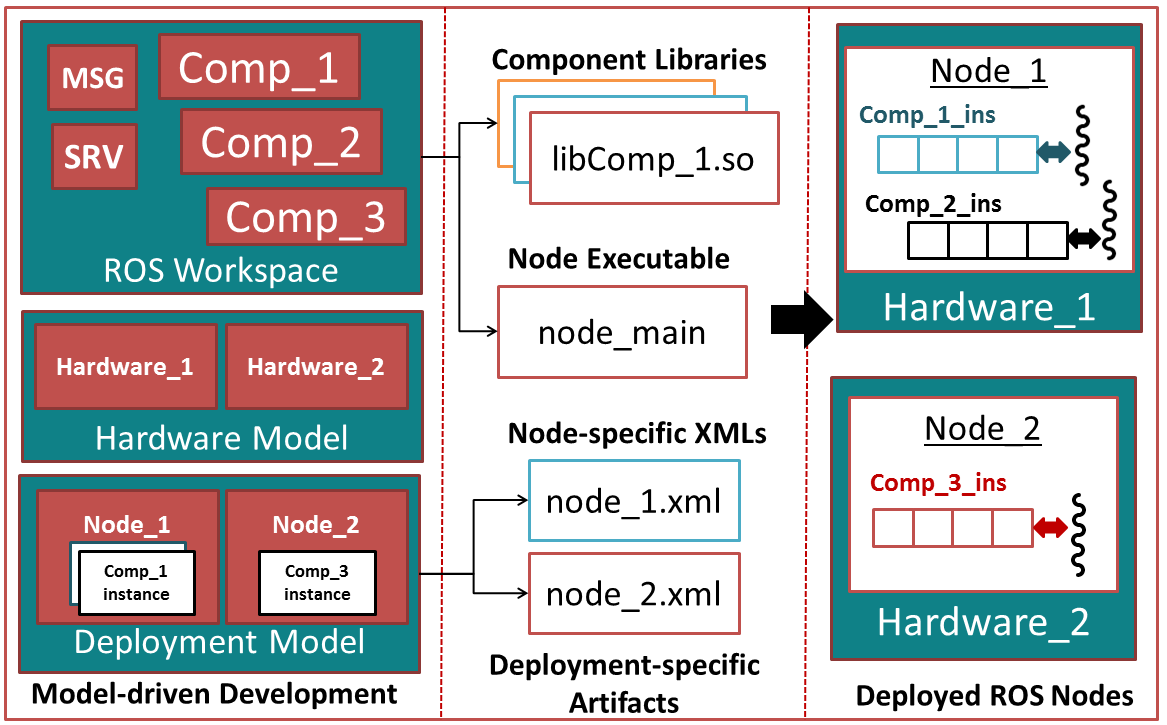
\includegraphics[width=\textwidth]{workflow}
    \caption{ROSMOD Deployment Framework}
    \label{fig:rosmod_deployment}
\end{figure}
 
In the above architecture, the deployment needs three primary ingredients: (1) the generic node executable, (2) dynamically loadable component libraries, and (3) an XML file for each ROS node in the deployment model. For each new node added to the deployment model, by merely regenerating the XML files, we can establish a new deployment. The ROS workspace is rebuilt only if new component definitions are added to the Software Model. This architecture not only accelerates the development process but also ensures a separation between the Software Model (i.e. the application structure) and deployment-specific concerns e.g. component instantiation inside ROS nodes.

\section{Evaluation of Timing Analysis Results}

Experimental validation should demonstrate that online measurements of the real-time system match with the timing analysis results in a way that the timing analysis results are always close but conservative. One of the biggest assumptions in our CPN work is the knowledge of worst-case execution times of the individual steps in the component operations. We have previously designed \cite{SEUS} a business-logic modeling grammar that captures the temporal behavior of component operations, especially WCET metrics for the different code blocks inside an operation. For example, consider a simple client-server example as shown in Figure \ref{fig:rmi_application}. The client component is periodically triggered by an internal timer and executes a synchronous remote method invocation to a remote server component. The interaction here demands that the client component be blocked for the duration of time it takes the server to receive the operation, process its message queue, execute the relevant callback, and respond with output. 

Note that in Figure \ref{fig:rmi_application}, we only annotate isolated code blocks that take a fixed amount of execution time on a specific hardware architecture. These are the only measurements that we can reliably make with repeated testing and instrumentation. The client-side blocking delay is not measured because the number of factors responsible for this delay are numerous e.g. server's message queue state, scheduling non-determinism, network delays etc. In order to be able to predict this delay, we need to use state space analysis and search through the tree of possible executions to identify the worst-case blocking delay. This also means that our CPN model must capture and account for such delay-causing factors. 

\begin{figure}[ht]
	\centering
	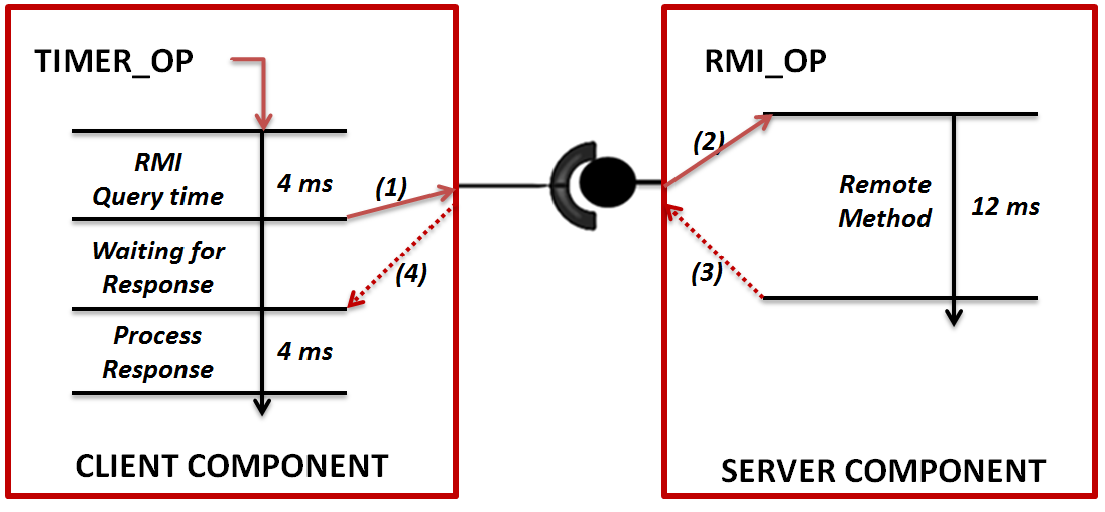
\includegraphics[width=\textwidth]{rmi_application}
	\caption{RMI Application}
	\label{fig:rmi_application}
\end{figure}

WCET of component operational steps needs to be measured by having the component operation execute at real-time priority with no other component threads intervening this process. This measurement gives us a \emph{pure execution time} of the code block. The process must be repeated for all component operations to obtain meaningful worst-case estimates that are tailored to the target platform. Obtaining the WCET values by this method is not only more realistic but also an accurate representation of the target system. Once these individual numbers are obtained, the values are plugged into the CPN through our business-logic models. 

The remainder of this section presents various primitive interaction patterns and assemblies that have been evaluated. The results are restricted to simple cases, though we have tested on medium-to-large scale examples spanning 25-30 computing nodes, and with up to a 100 components. The scalability of our model, however, is not within the scope of this paper as we have previously evaluated this metric \cite{SEUS}. As mentioned earlier, in all of our tests, we use the ROS \cite{ROS} middleware and our ROSMOD \cite{kumarROSMOD} component model. 

\subsection{Client-Server Interactions}

As shown in Figure \ref{fig:rmi_application}, a simple client server example involves a periodically triggered client component that fetches data from a remote server. Figure \ref{fig:client-server} shows our experimental trace of a simple distributed client-server sample. The client (client\_timer\_operation) is triggered every 500 ms, and performs floating-point calculations in a loop requiring the services of a remote operation.  %The loop bound is a random variable having a uniform distribution between some peak iteration count and 60\% of this peak. 
The server (Power\_operation) periodically receives this operation request and responds to it, taking about 1.2s to complete each operation instance. In this experiment, these component threads are running at high uninterrupted real-time priorities. 

\begin{figure}[h]
	\centering
	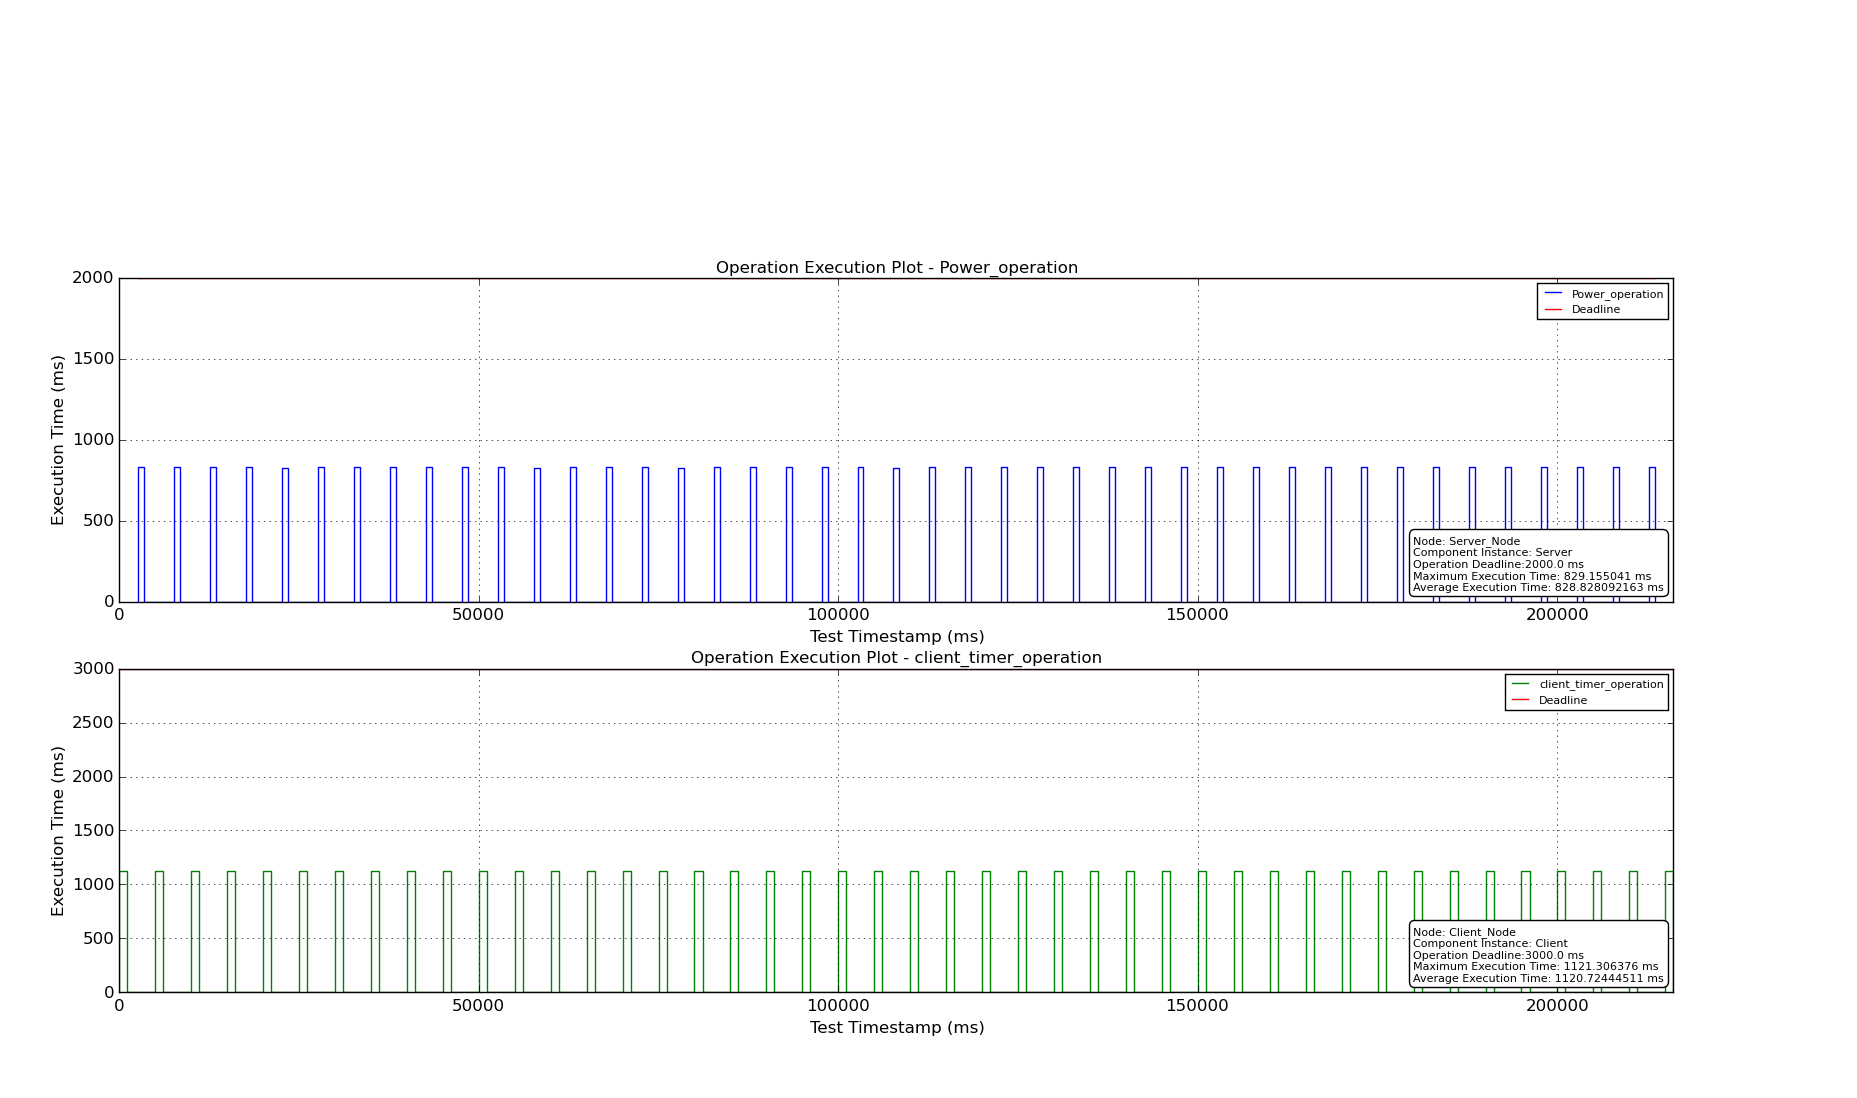
\includegraphics[width=\textwidth]{client-server}
	\caption{Experimental Observation: Client-Server Interactions}
	\label{fig:client-server}
\end{figure}

Figure \ref{fig:client-server-cpn} shows the execution time plot derived from our CPN. As expected, since there are no other interruptions on the server side, the server is able to promptly respond to the client.

\begin{figure}[h]
	\centering
	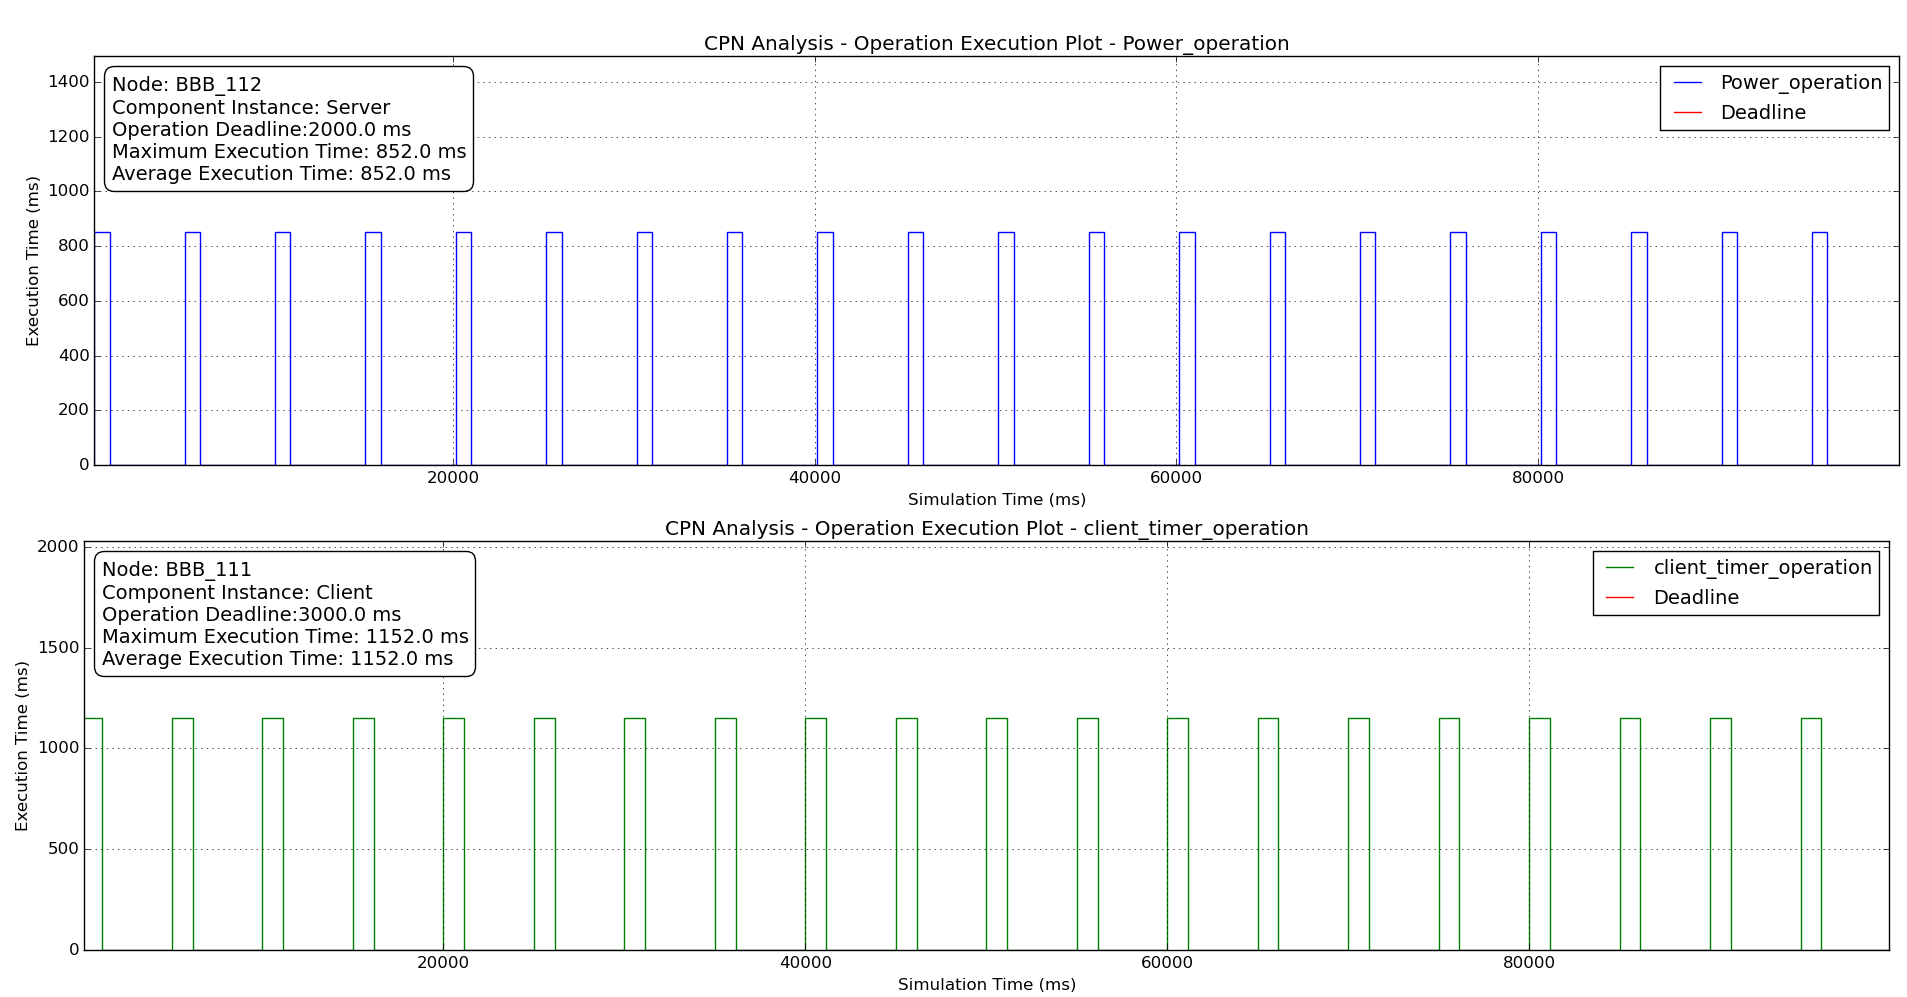
\includegraphics[width=\textwidth]{client-server-cpn}
	\caption{CPN Analysis Results: Client-Server Interactions}
	\label{fig:client-server-cpn}
\end{figure}


\subsection{Publish-Subscribe Interactions}

Similar to the earlier example, consider a simple anonymous publish-subscribe interaction. A publisher is periodically triggered by a timer when this component broadcasts a message on a topic. A subscribing component receives this message and performs some computation.

\begin{figure}[h]
	\centering
	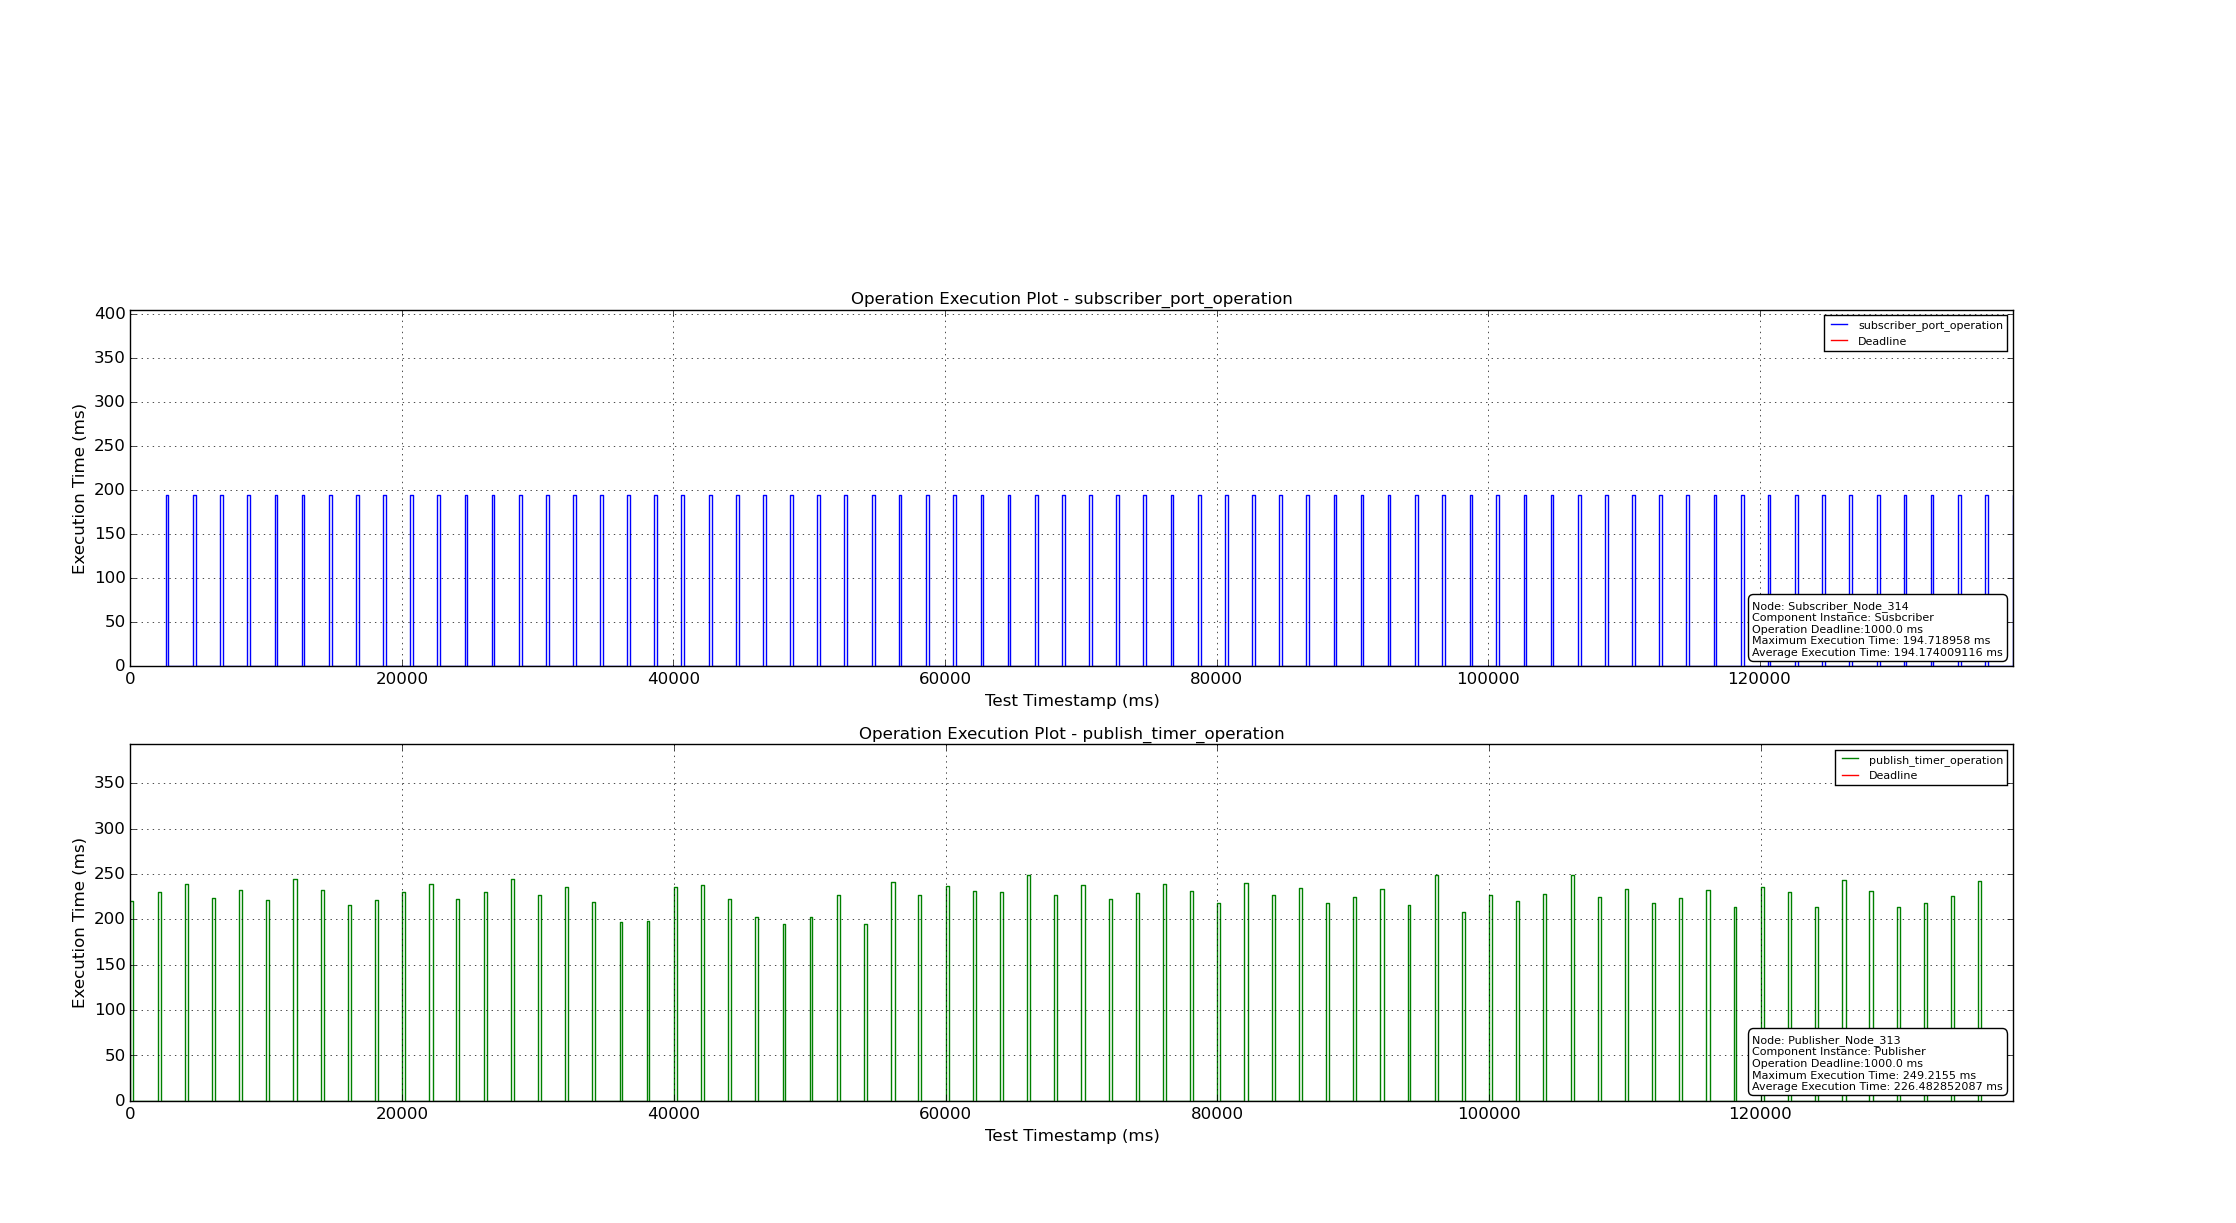
\includegraphics[width=\textwidth]{publish-subscribe}
	\caption{Experimental Observation: Publish-Subscribe Interactions}
	\label{fig:publish-subscribe}
\end{figure}

Figure \ref{fig:publish-subscribe} shows our testbed observations and Figure \ref{fig:publish-subscribe-cpn} shows our CPN analysis results. As evident, the CPN results closely match and validate this sample. 

\begin{figure}[h]
	\centering
	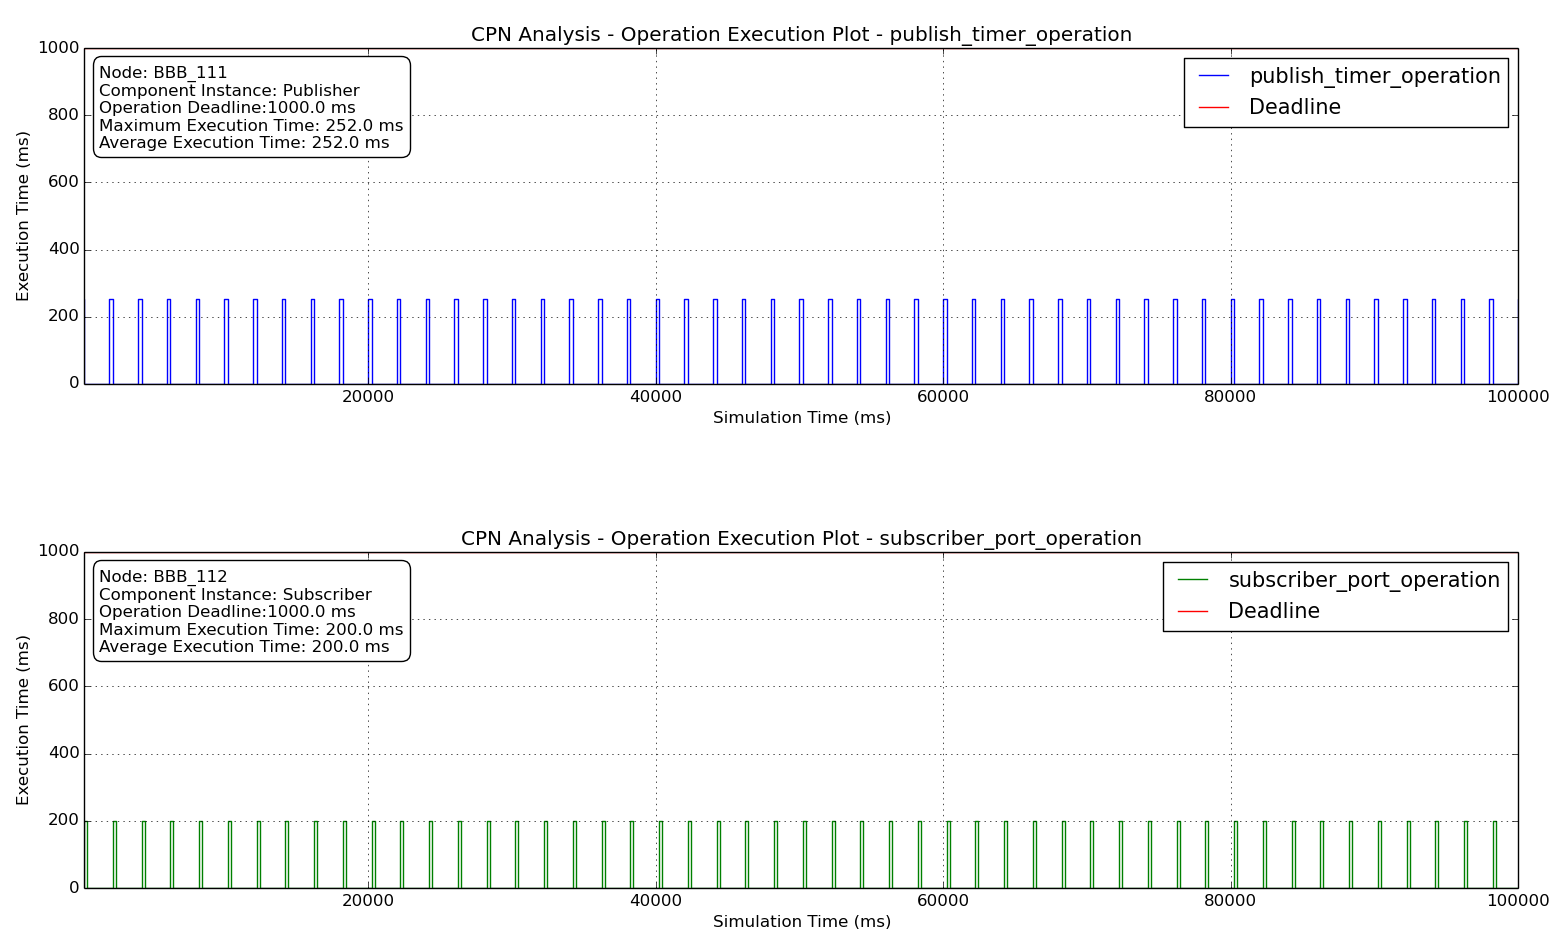
\includegraphics[width=\textwidth]{publish-subscribe-cpn}
	\caption{CPN Analysis Results: Publish-Subscribe Interactions}
	\label{fig:publish-subscribe-cpn}
\end{figure}

\subsection{Trajectory Planner}

In the past \cite{kumar2014colored}, we have used a \emph{Trajectory Planner} deployment to illustrate the utility of our state space analysis. Figure \ref{fig:trajectory-planner} shows the execution time plot of this sample. A Sensor component is periodically triggered every second by the \emph{sensor\_timer} at which point it publishes a notification to the Trajectory Planner, alerting the planner of new sensor state. The planner component receives this notification on its \emph{state\_subscriber}. On receiving this message, the planner executes a remote method invocation to the \emph{compute} server located in the Sensor, blocked and waiting for a response. At this point, the \emph{compute\_operation} is executed on the Sensor which returns the updated sensor state. This unblocks the planner component which uses the new sensor state to perform trajectory planning tasks. 


\begin{figure}[h]
	\centering
	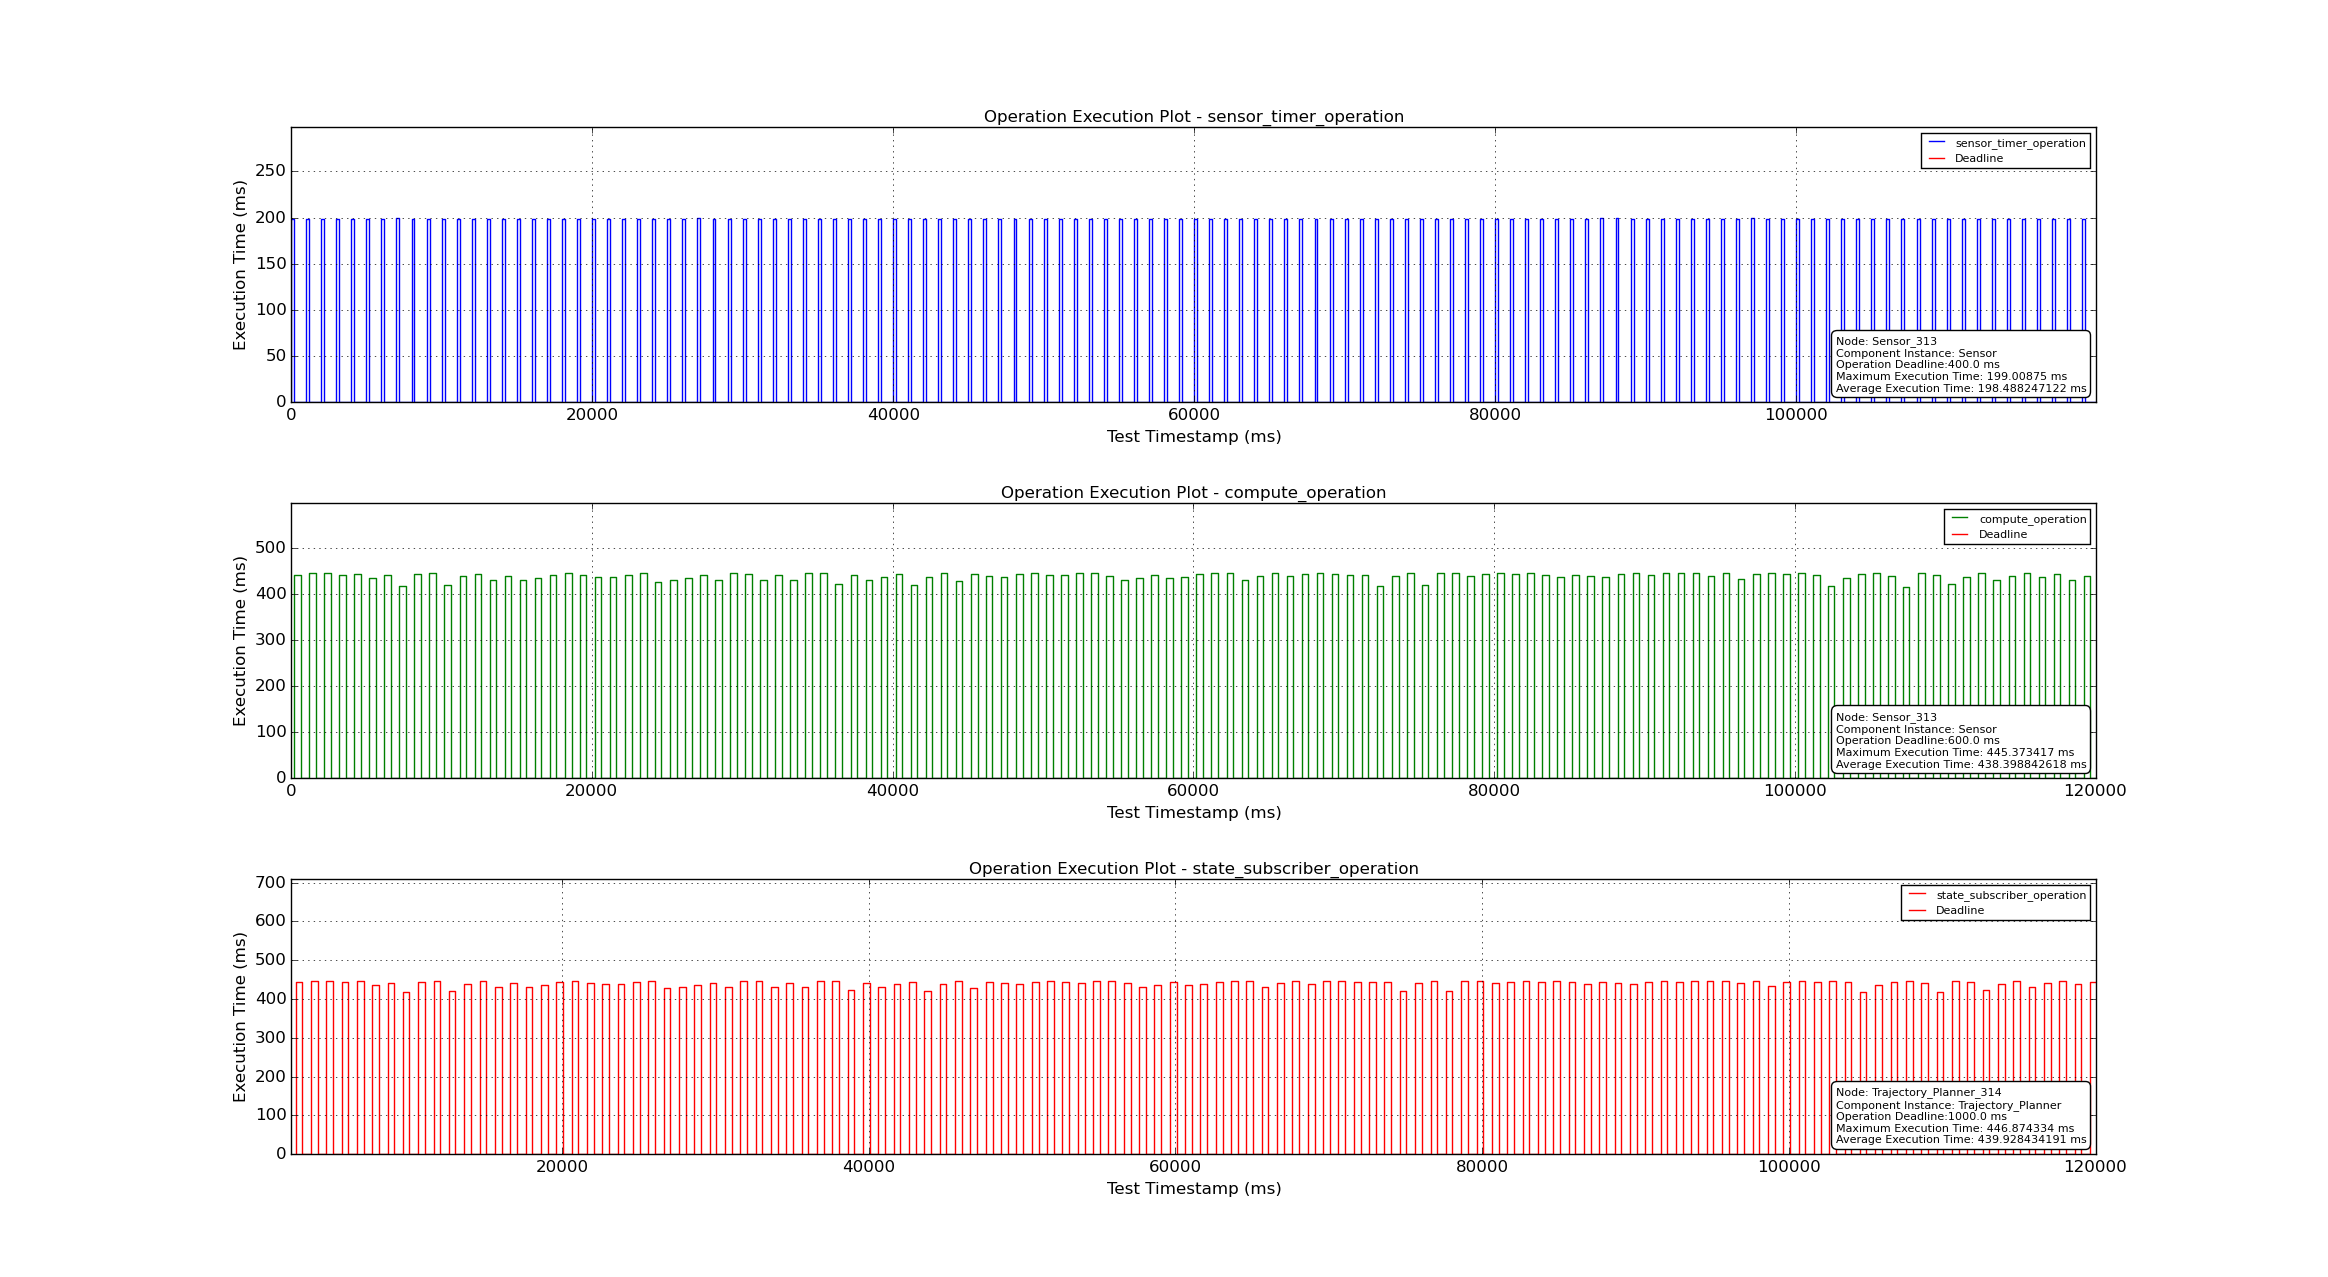
\includegraphics[width=\textwidth]{trajectory-planner}
	\caption{Experimental Observation: Trajectory Planner}
	\label{fig:trajectory-planner}
\end{figure}

This is a common interaction pattern in Cyber-Physical systems since embedded sensors are updated at a much higher frequency than a path planning entity. Thus, the planner can query the sensor at a lower rate to sample the sensor state. In this example, the planner is matching the frequency of the sensor since the execution cost is low. However, when more components are added to this deployment, the planner would have to fetch sensor state less frequently so as to not affect other system-level deadlines.  

\begin{figure}[h]
	\centering
	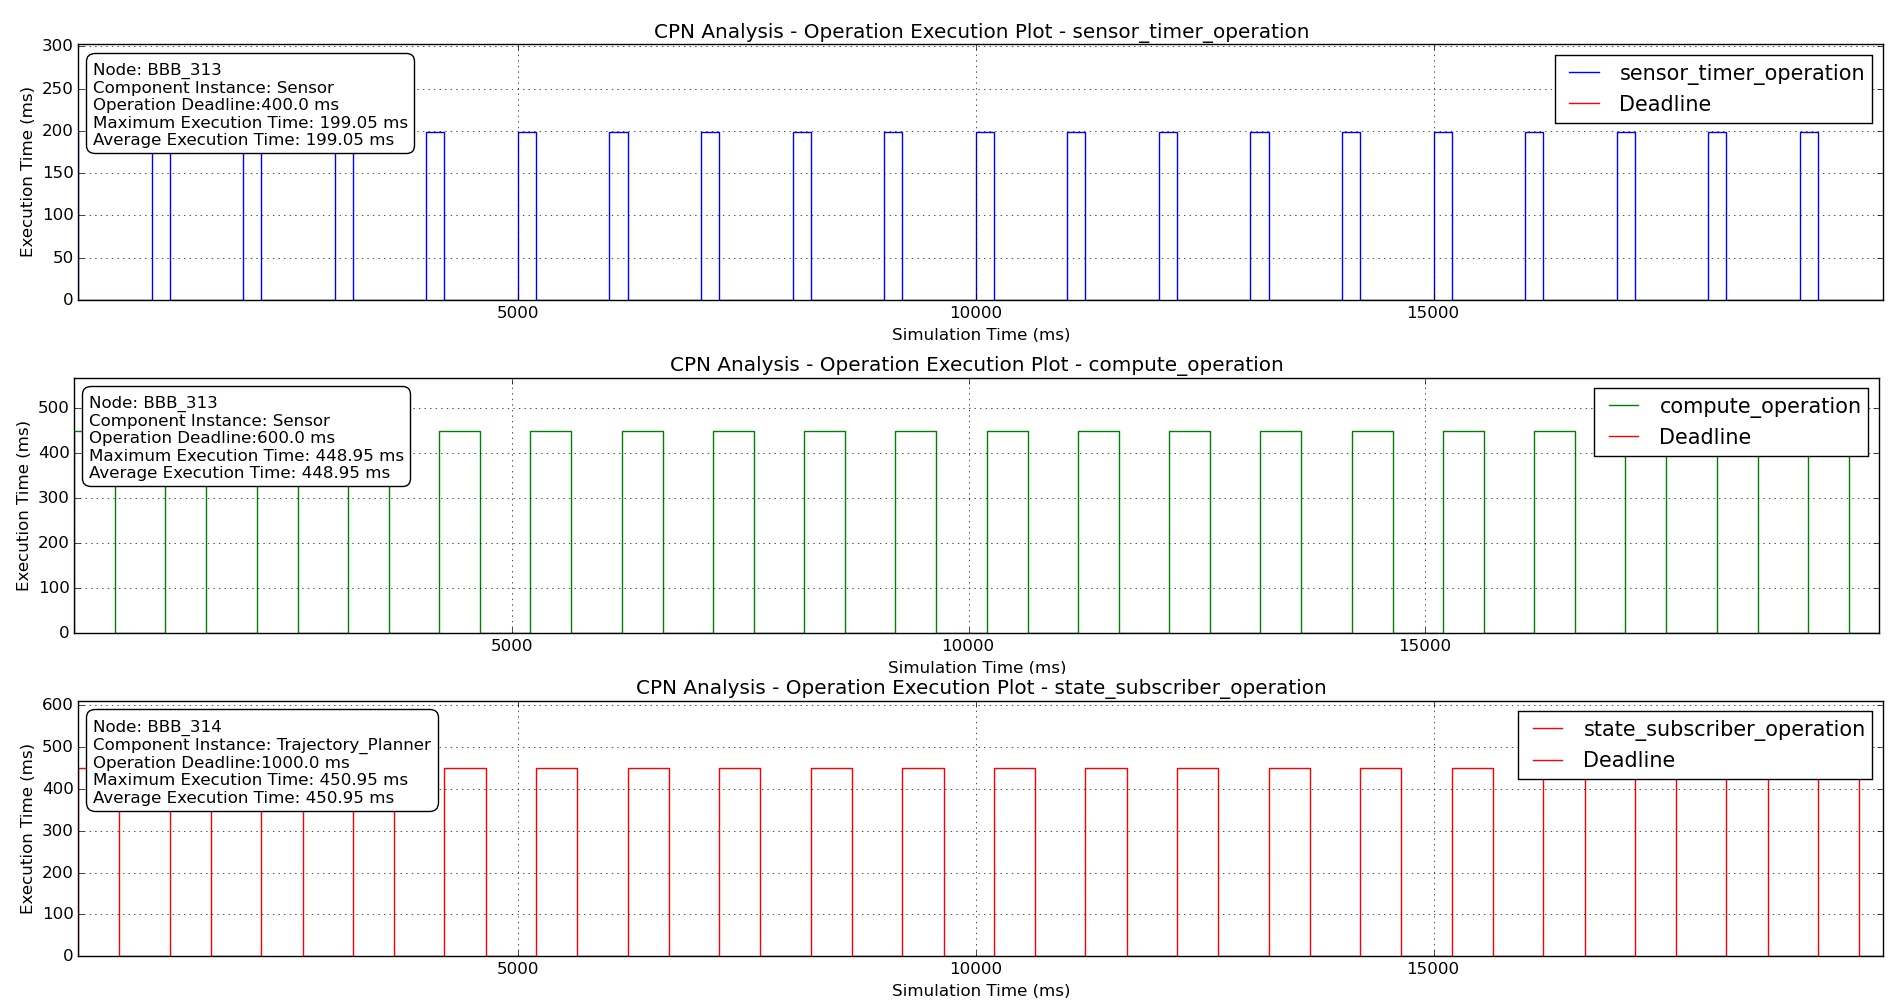
\includegraphics[width=\textwidth]{trajectory-planner-cpn}
	\caption{CPN Analysis Results: Trajectory Planner}
	\label{fig:trajectory-planner-cpn}
\end{figure}

\subsection{Time-triggered Operations}

Time-triggered operations are an integral part of our component model. DREMS components are dormant by default. A timer has to trigger a inactive component for all subsequent interactions to happen. Since the DREMS component model supports various scheduling schemes on a single component message queue, this following test evaluates a priority first-in first-out (PFIFO) scheme. Multiple timers are created in a single component, each with a unique priority and period. A timer with a high frequency is assigned a high priority. Figure \ref{fig:periodic-timers} shows our experimental observations on a 5-timer example. 

Since ROSMOD components are associated with a single executor thread and component operations are also non-preemptive, a low-priority operation could theoretically run forever, starving a higher priority operation from ever executing, leading to deadline violations e.g. \emph{Timer\_1\_operation} can affect all other higher priority timers. Figure \ref{fig:periodic-timers-cpn} shows our CPN prediction where such a scenario is evident. It can be seen that \emph{Timer\_5\_operation}, the timer with the highest priority is periodically seeing spikes in execution time, courtesy of other lower priority operations consuming CPU without preemption.

It must be noted here that the execution time values assigned to each timer operation in our CPN is the pure execution time i.e. the time taken for each timer operation to execute on the target CPU without interruption. This is the case for all operational execution times injected into the analysis model. If this is not done, then due to scheduling delays and interaction patterns, the CPN results will become gross overestimates. 

\begin{figure}[h]
	\centering
	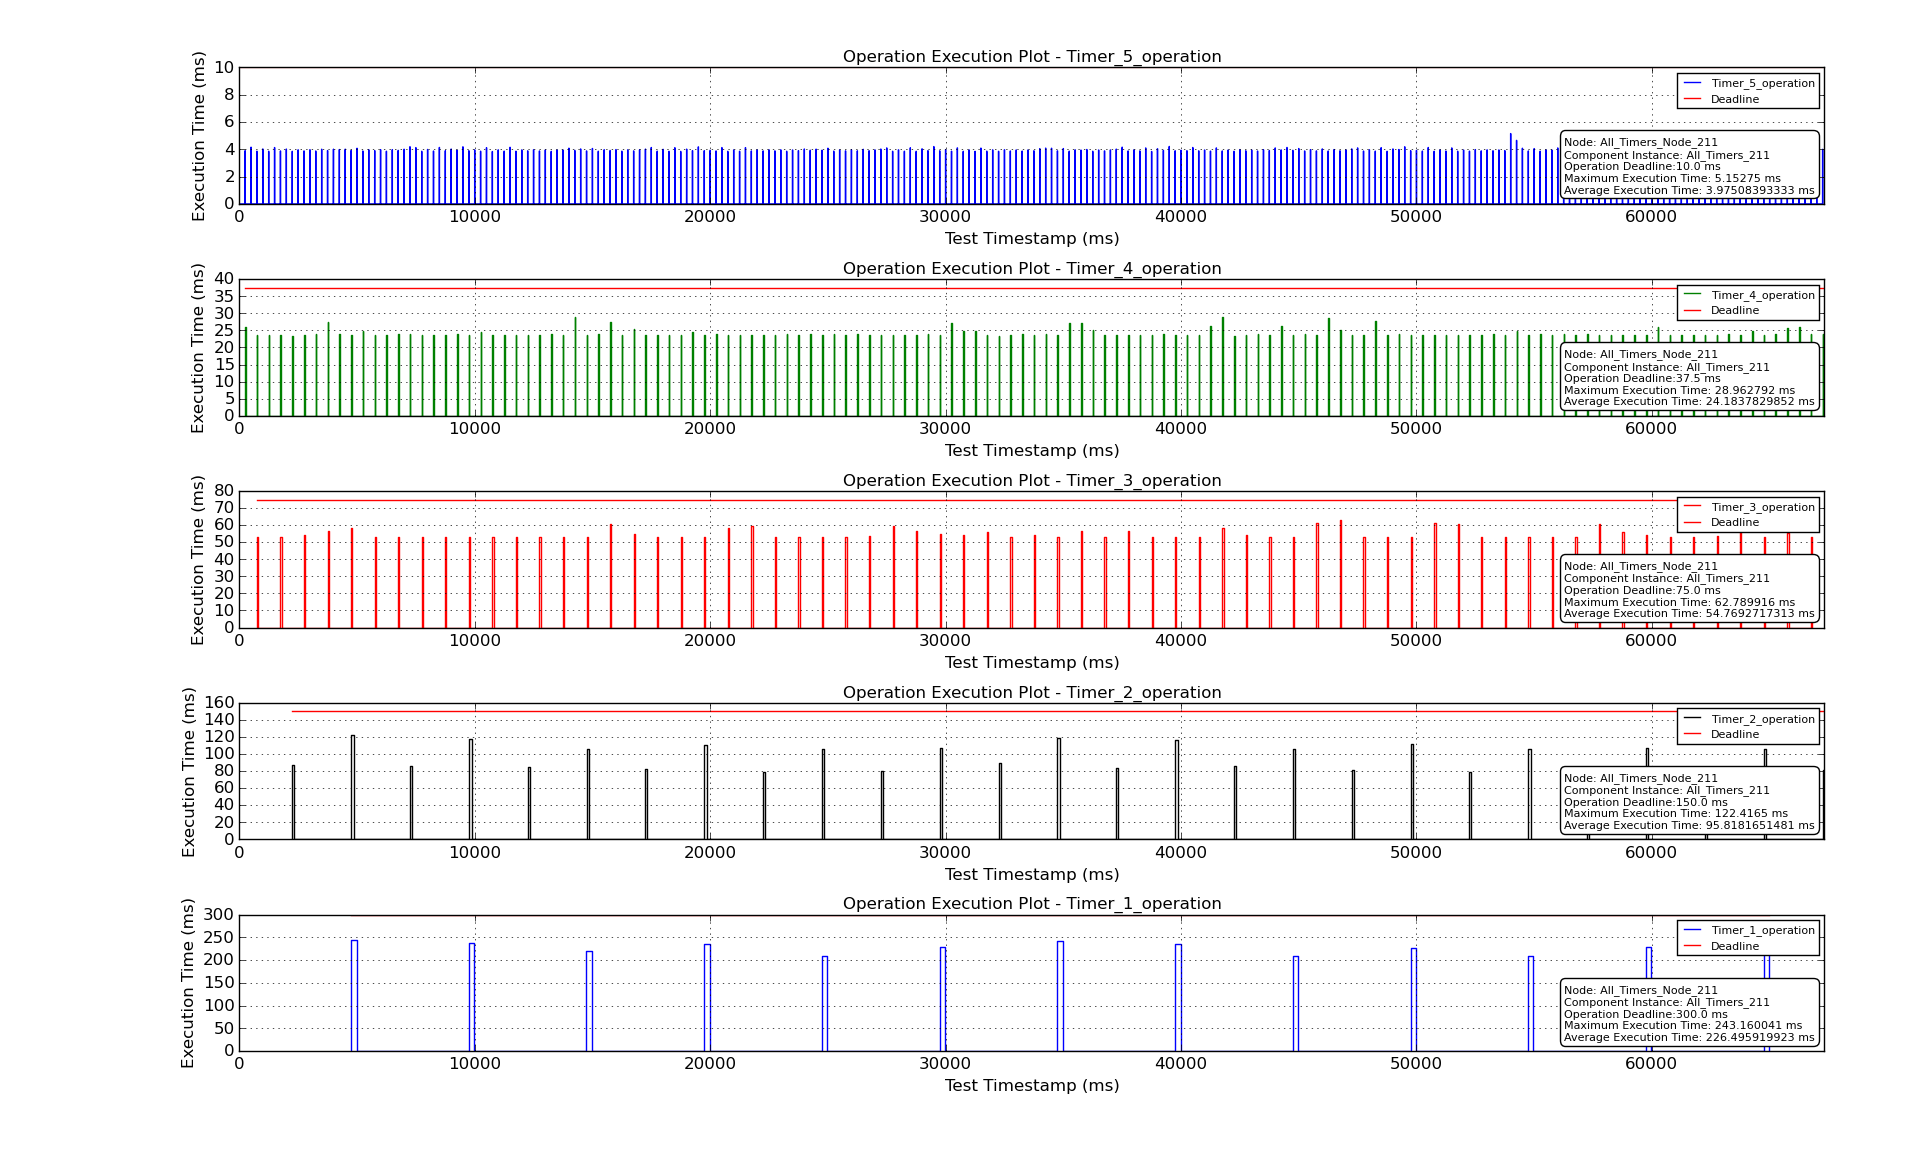
\includegraphics[width=\textwidth]{periodic-timers}
	\caption{Experimental Observation: Periodic Timers}
	\label{fig:periodic-timers}
\end{figure}

\begin{figure}[h]
	\centering
	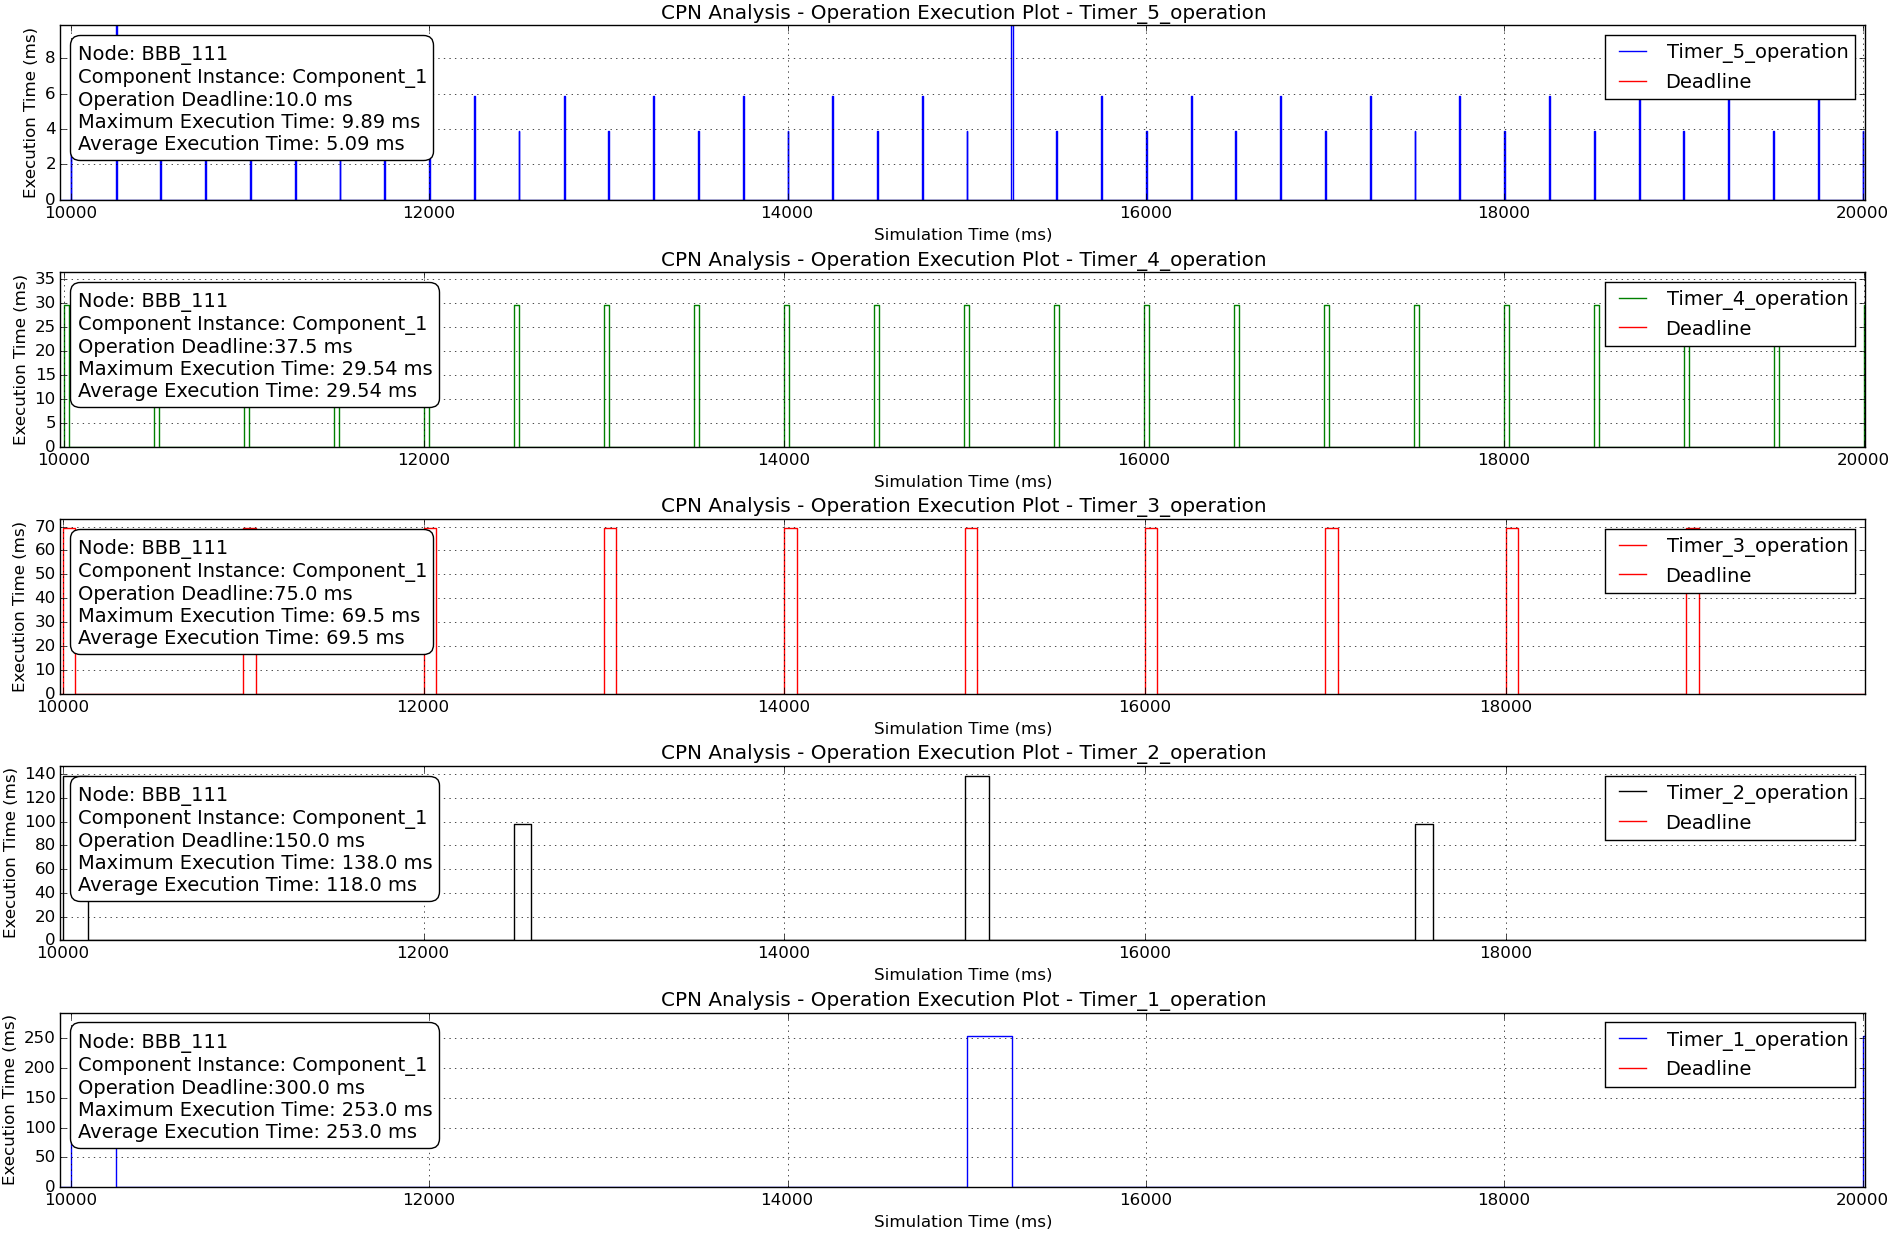
\includegraphics[width=\textwidth]{periodic-timers-cpn}
	\caption{CPN Analysis Results: Periodic Timers}
	\label{fig:periodic-timers-cpn}
\end{figure}

\subsection{Long-Running Operations}

Our ROSMOD component model implements a non-preemptive component operation scheduling scheme. A component operation that is in the queue, regardless of its priority, must wait for the currently executing operation to run to completion. This is a strict rule for operation scheduling and does not work best in all system designs e.g. in a long-running computation-intensive application, rejuvenating the executing operation periodically and restarting it at a previous checkpoint increases the likelihood of successfully completing the application execution. In applications executing long-running artificial intelligence (AI) search algorithms e.g. flight path planning algorithms, the computation should not hinder the prompt response requirements of highly critical operation requests such as sudden maneuver changes. Our ROSMOD component model does not support the \emph{cancellation} of long-running component operations to service other highly critical operations waiting in the queue. With a few minor modifications to our scheduling schemes, long running operations can, however, be suspended if a higher priority waiting operation requires service. With these additions, we are able to model and analyze component-based systems that support long-running operations, with checkpoints, enabling the novel integration of AI-type algorithms into our design and analysis framework. 

\subsubsection{Challenges}

One of the primary challenges here is to identify the semantics of a long-running component operation i.e. the scenarios under which the component operations scheduler suspends a cooperating long-running operation in favor of some other operation waiting in the queue. If a long-running computation is modeled as a sequence of execution steps with bounded checkpoints, then the operation would execute one step at a time and suspend at such checkpoints if necessary. An important challenge here is accurately identifying the priority difference between the long-running operation and the waiting operation. If the long-running operation is one checkpoint away from completion e.g. 100-200 ms of execution time, then strictly following our suspension rules would not be the most prudent choice since this operation is almost complete. However, if the waiting operation is a critical one, then regardless of the state of the long-running operation, the executing operation must be suspended. Secondly, the modeled long-running computation semantics must be incorporated into our component model so that any analysis results obtained can be suitably validated. 

\begin{figure}[h]
	\centering
	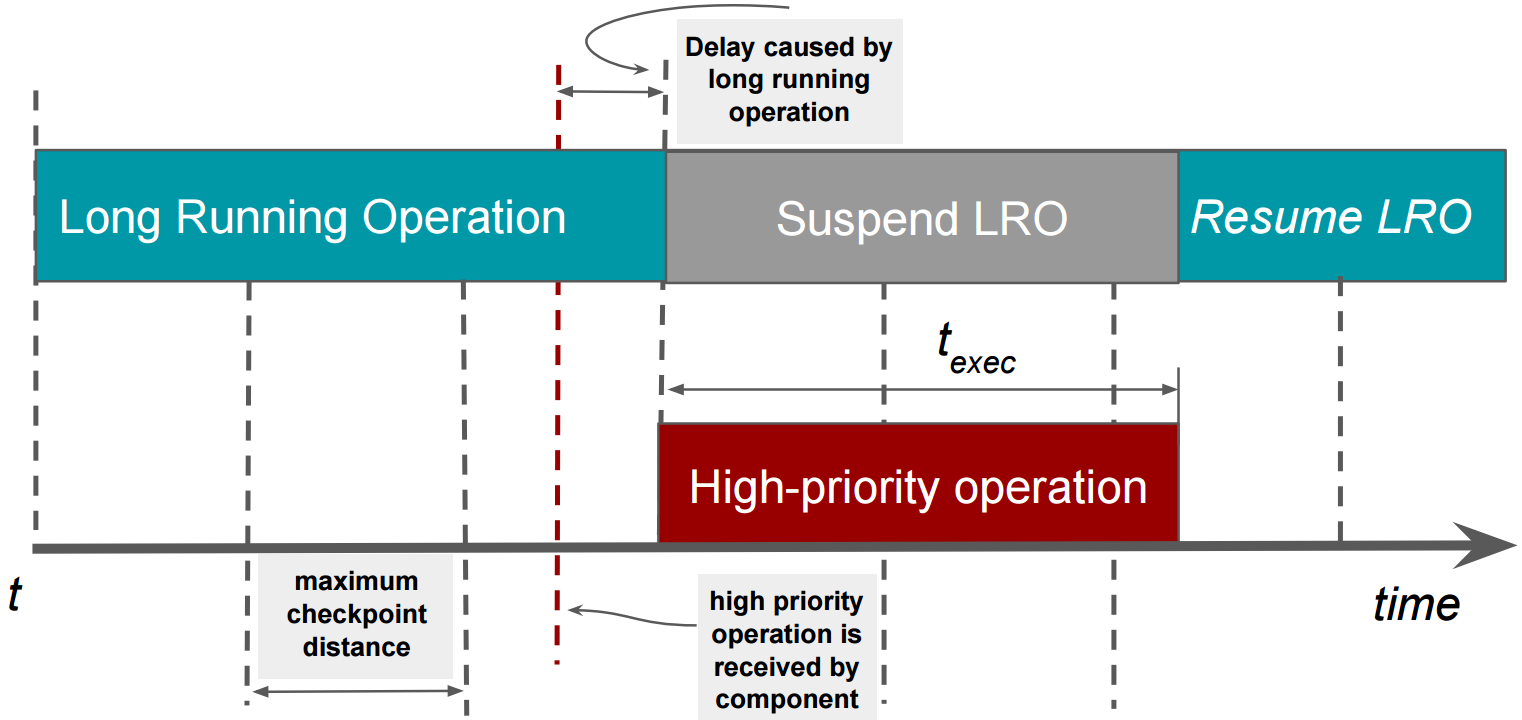
\includegraphics[width=\textwidth]{lro-semantics}
	\caption{Long Running Operations - Timing Diagram}
	\label{fig:lro-semantics}
\end{figure}

\subsubsection{Implementation and Results}

In each long-running operation, we, therefore, include a synchronous \emph{checkpoint step}, as shown in Figure \ref{fig:lro-semantics}. The only assumption we make about this long-running operation is the periodicity of these checkpoint steps i.e. we know how frequently a new checkpoint is reached and we assume that the search algorithm used by the long-running operation is capable of reaching a safe state (the checkpoint) before suspending itself if required. If a higher priority operation is ready and waiting in the queue, the long-running operation runs till the next checkpoint is reached, then suspends. The higher priority operation is then processed. Figure \ref{fig:three-components-lro-rosmod} shows the \emph{Software Model} for a component assembly with long running operations.

\begin{figure}[h]
	\centering
	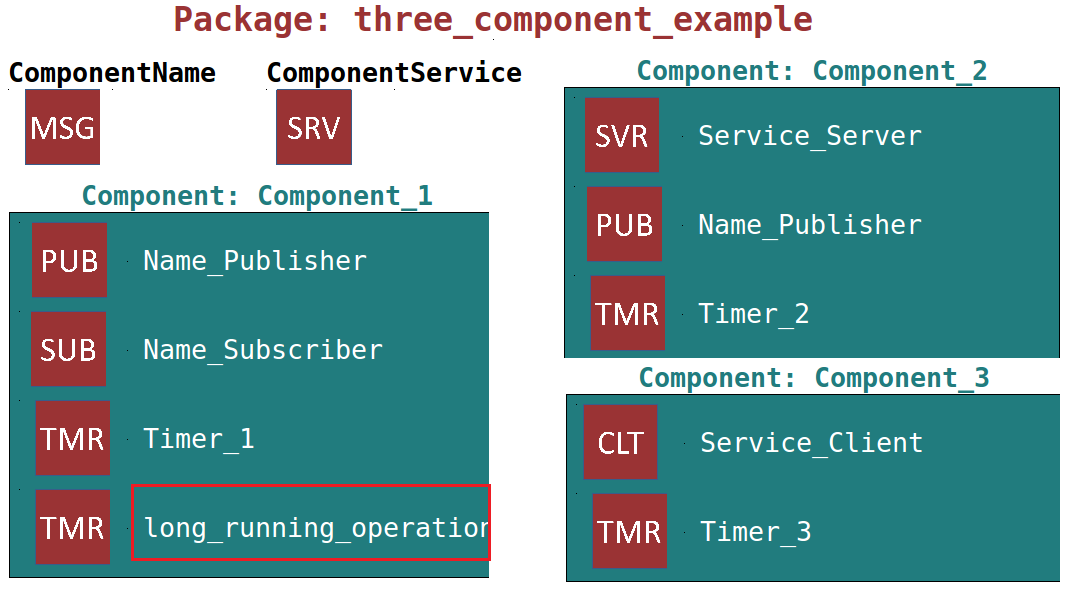
\includegraphics[width=\textwidth]{three-components-lro-rosmod}
	\caption{Long Running Operation - Software Model}
	\label{fig:three-components-lro-rosmod}
\end{figure}

The assembly consists of three components. Components \emph{Component\_1} and \emph{Component\_2} periodically publish on the \emph{ComponentName} message. \emph{Component\_3} periodically queries the server in \emph{Component\_2}. During these interactions, \emph{Component\_1} is performing a long running operation, the duration of which, is magnitudes larger than the average execution time of all other operations. Figure \ref{fig:three-components-lro} shows the execution time plot of this scenario, as measured on our testbed. 

For the CPN analysis, in order to obtain pure execution times of all these operations, each operation on each component is executed as a stand-alone function on the hardware. This way, we know the average and worst-case execution times of all operational steps with minimal interruptions. These numbers are injected into our generated CPN and state space analysis is performed. Figure \ref{fig:three-components-lro-cpn} shows our CPN analysis results for the same assembly.

\begin{figure}[h]
	\centering
	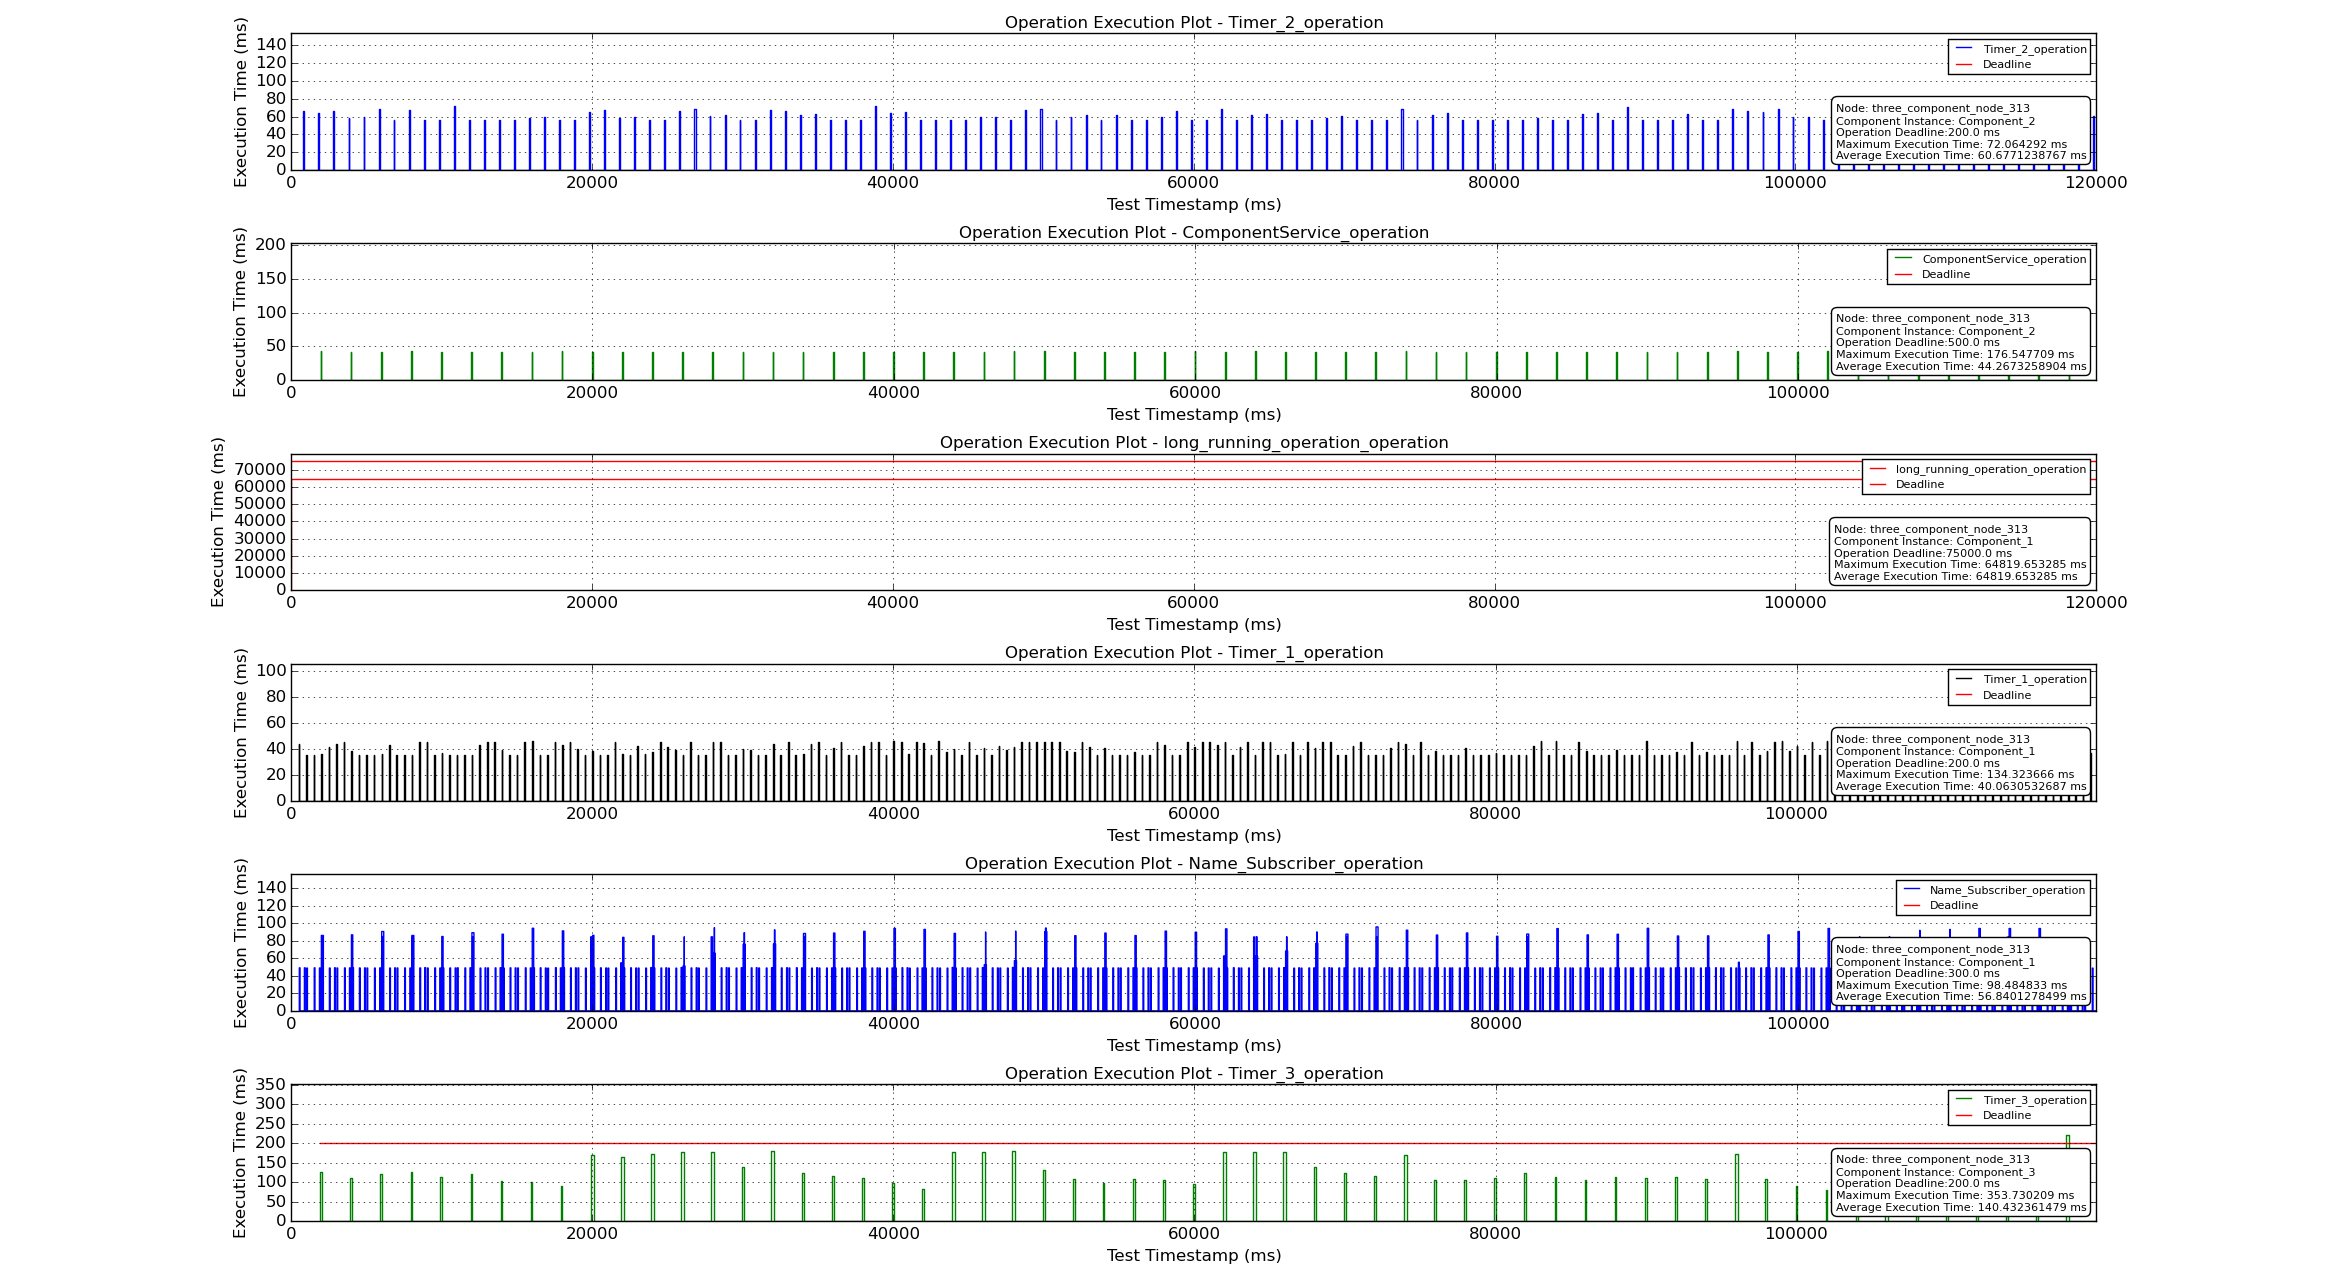
\includegraphics[width=\textwidth]{three-components-lro}
	\caption{Experimental Observation: Composed Component Assembly}
	\label{fig:three-components-lro}
\end{figure}

\begin{figure}[h]
	\centering
	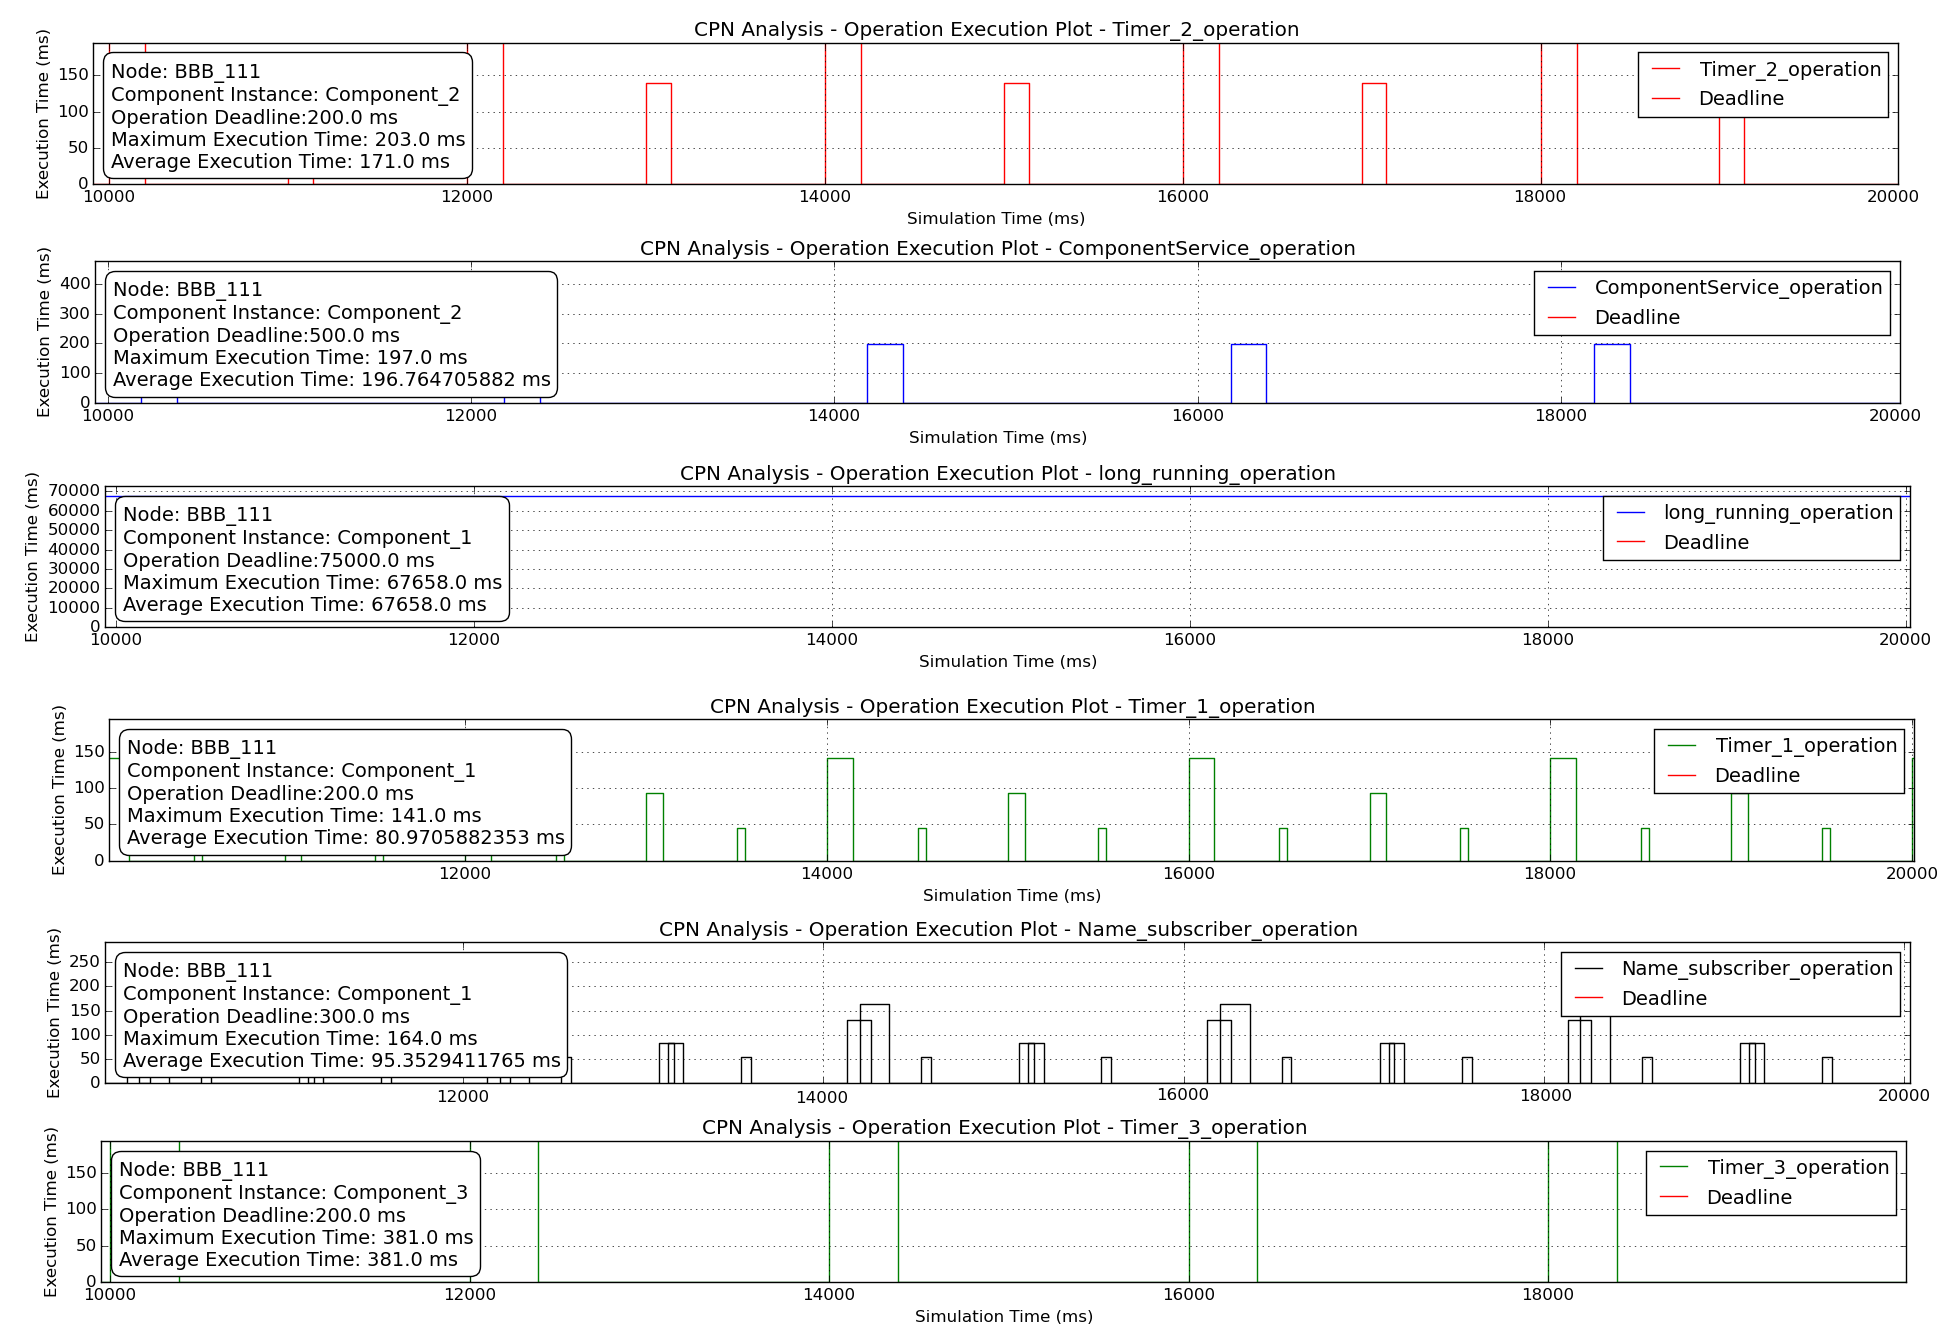
\includegraphics[width=\textwidth]{three-components-lro-cpn}
	\caption{CPN Analysis Results: Composed Component Assembly}
	\label{fig:three-components-lro-cpn}
\end{figure}

\subsection{Cyber-Physical Systems: Autonomous Ground Support Equipment (AGSE) Robot}

This section briefly describes an Autonomous Ground Support Equipment
(AGSE) robot that we designed, built, and deployed for the 2014-2015
NASA Student Launch Competition \cite{NASA_SL}. Special emphasis is
given to the value of a rapid system prototyping methodology in the
design process and how it allowed the AGSE to overcome many of the
challenges and problems encountered during the competition.  We also use
this example as our cyber-physical system for timing analysis.

The NASA Student Launch Initiative \cite{NASA_SL} is a research-based
competition partnered with NASA's Centennial Challenges, and aims to
stimulate rapid, low-cost development of rocket propulsion and space
exploration systems.  Both collegiate and non-academic teams
participate in the 8-month competition cycle composed of design,
fabrication, and testing of flight vehicles, payloads, and ground
support equipment.

The purpose of the 2014-2015 competition was to simulate a Mars Ascent
Vehicle (MAV) and to perform a sample recovery from the Martian
surface. The requirements for this simulation were twofold: (1) Design
and deploy a system termed the Autonomous Ground Support Equipment
(AGSE) that independently retrieves a sample off the ground and stores
it in the payload bay of a rocket, and (2) launch the rocket to an
altitude of 3000 ft. before safely recovering the sample.

The sample retrieval was accomplished using a robotic arm with
computer vision to find the sample and identify its orientation. After
successfully acquiring the sample, the system will then search for the
payload bay, identify its orientation, and place the sample within it.
The robot arm itself is a simple crane-style device akin to a
pick-and-place robot with a four-pronged gripper as the end effector.
It was designed to have a cylindrical workspace in order to most
efficiently access the ground around the system and rocket. It starts
in a known position and incrementally scans its workspace using a
built in camera. Image processing is performed to identify key
environmental features such as the sample and payload bay.  The
control flow in the AGSE software is shown in Figure
\ref{fig:AGSE-FlowChart}.

\begin{figure}[h]
	\centering
	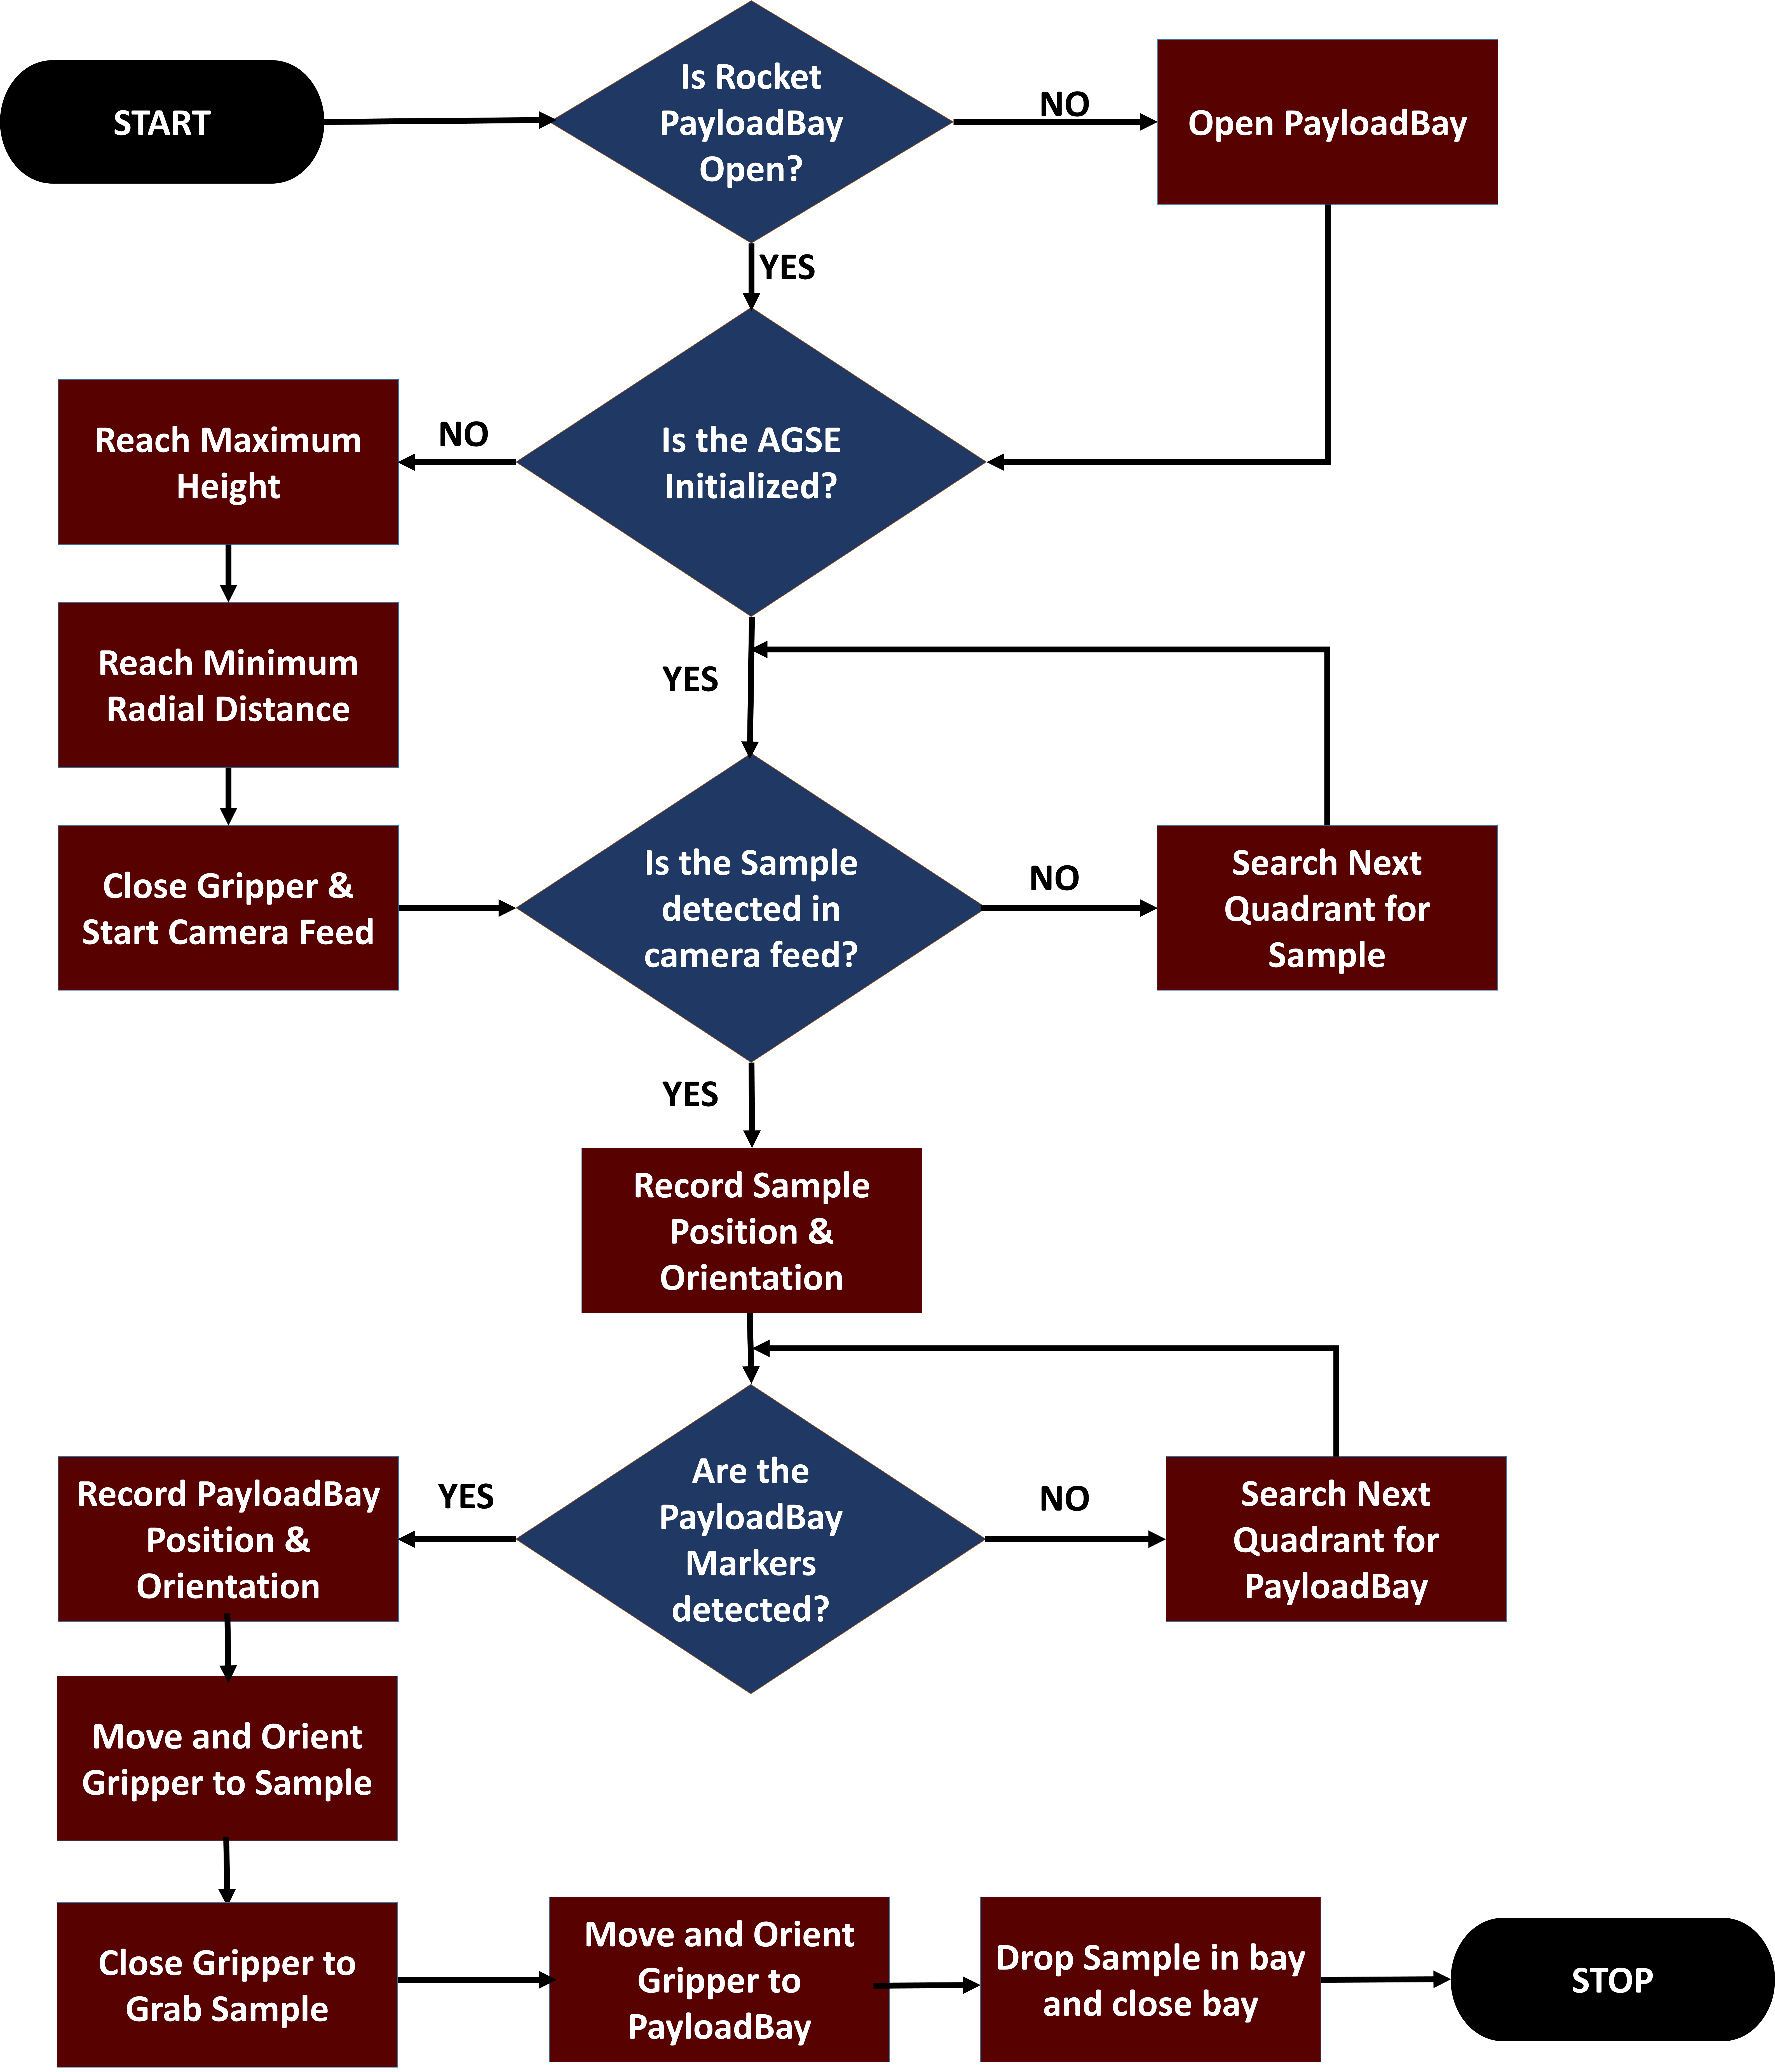
\includegraphics[width=0.8\textwidth]{AGSE-FlowChart.png}
	\caption{AGSE Control Flow Chart}
	\label{fig:AGSE-FlowChart}
\end{figure}

While the driving requirements of the competition were fixed, many of
the minor rules regarding AGSE performance, behavior, and safety
requirements evolved and were augmented throughout the course of the
competition. The volatile nature of these rules combined with the
short eight month duration of the build cycle precipitated the need
for rapidly adjustable design and fabrication processes. As such, an
iterative, modular, design-build-test approach was implemented in
order to concurrently develop as many components of the hardware and
software systems as possible. An initial AGSE prototype was
conceptualized from off-the-shelf components and the mechanical and
software systems were built in parallel, integrated, and tested. These
preliminary results were then used in future development to produce a
more ideal structure with greater positional accuracy and system
robustness.  Due to the modular nature of the system's design, it was
not necessary to immediately build a completely new second system, so
incremental improvements could be made on a specific subsystem (such
as the robot's gripper, any single degree of freedom, image
processing, motor control, etc.) as the design evolved.

\subsubsection{Distributed Deployment}

The AGSE robot is controlled by a distributed set of embedded
controllers. Figure \ref{fig:AGSE_Deployment} shows the high-level
design for the deployment architecture. There are three embedded
devices, each with its own responsibilities.  The reasons for the use
of multiple embedded controllers cooperating was two-fold: 1) given
the design decision to fully automate the robot to search the
workspace for both the sample and the payload bay, we needed an
embedded processor capable of performing image-based object detection
and 2) given the design of the robot to search a workspace with the
given degrees of freedom, we needed an embedded processor with the
required available General Purpose Input/Output (GPIO) and Special
Function Input/Output (SFIO) pins. 

To meet the first requirement, we selected the NVIDIA Jetson TK1, which is an embedded ARM controller
with 4+1 ARM cores and 192 CUDA cores, that consumes 10 W or less.
We could not use the Jetson to meet the second requirement since it
does not support enough GPIO to control the linear actuators and
retrieve feedback from them.  Furthermore, it lacks SFIO for encoder
pulse decoding.  Therefore, a BeagleBone Black was selected for the
motor control interface board because it has specific hardware for
decoding quadrature encoded pulses (QEP) and enough available GPIO for
controlling the linear actuators and reading limit switches.

Since one of the secondary requirements of the competition governed
pause control and state feedback to the operator of the AGSE (during
the competition execution), a second BeagleBone Black was introduced
which served to provide mechanical safety switches for pausing the
AGSE, LED panels indicating the state of the AGSE, and a touchscreen
showing what the AGSE sees as it searches the workspace for the sample
and the payload bay.  This BeagleBone Black resides the User Interface
Panel (UIP).

\begin{figure}[h]
	\centering
	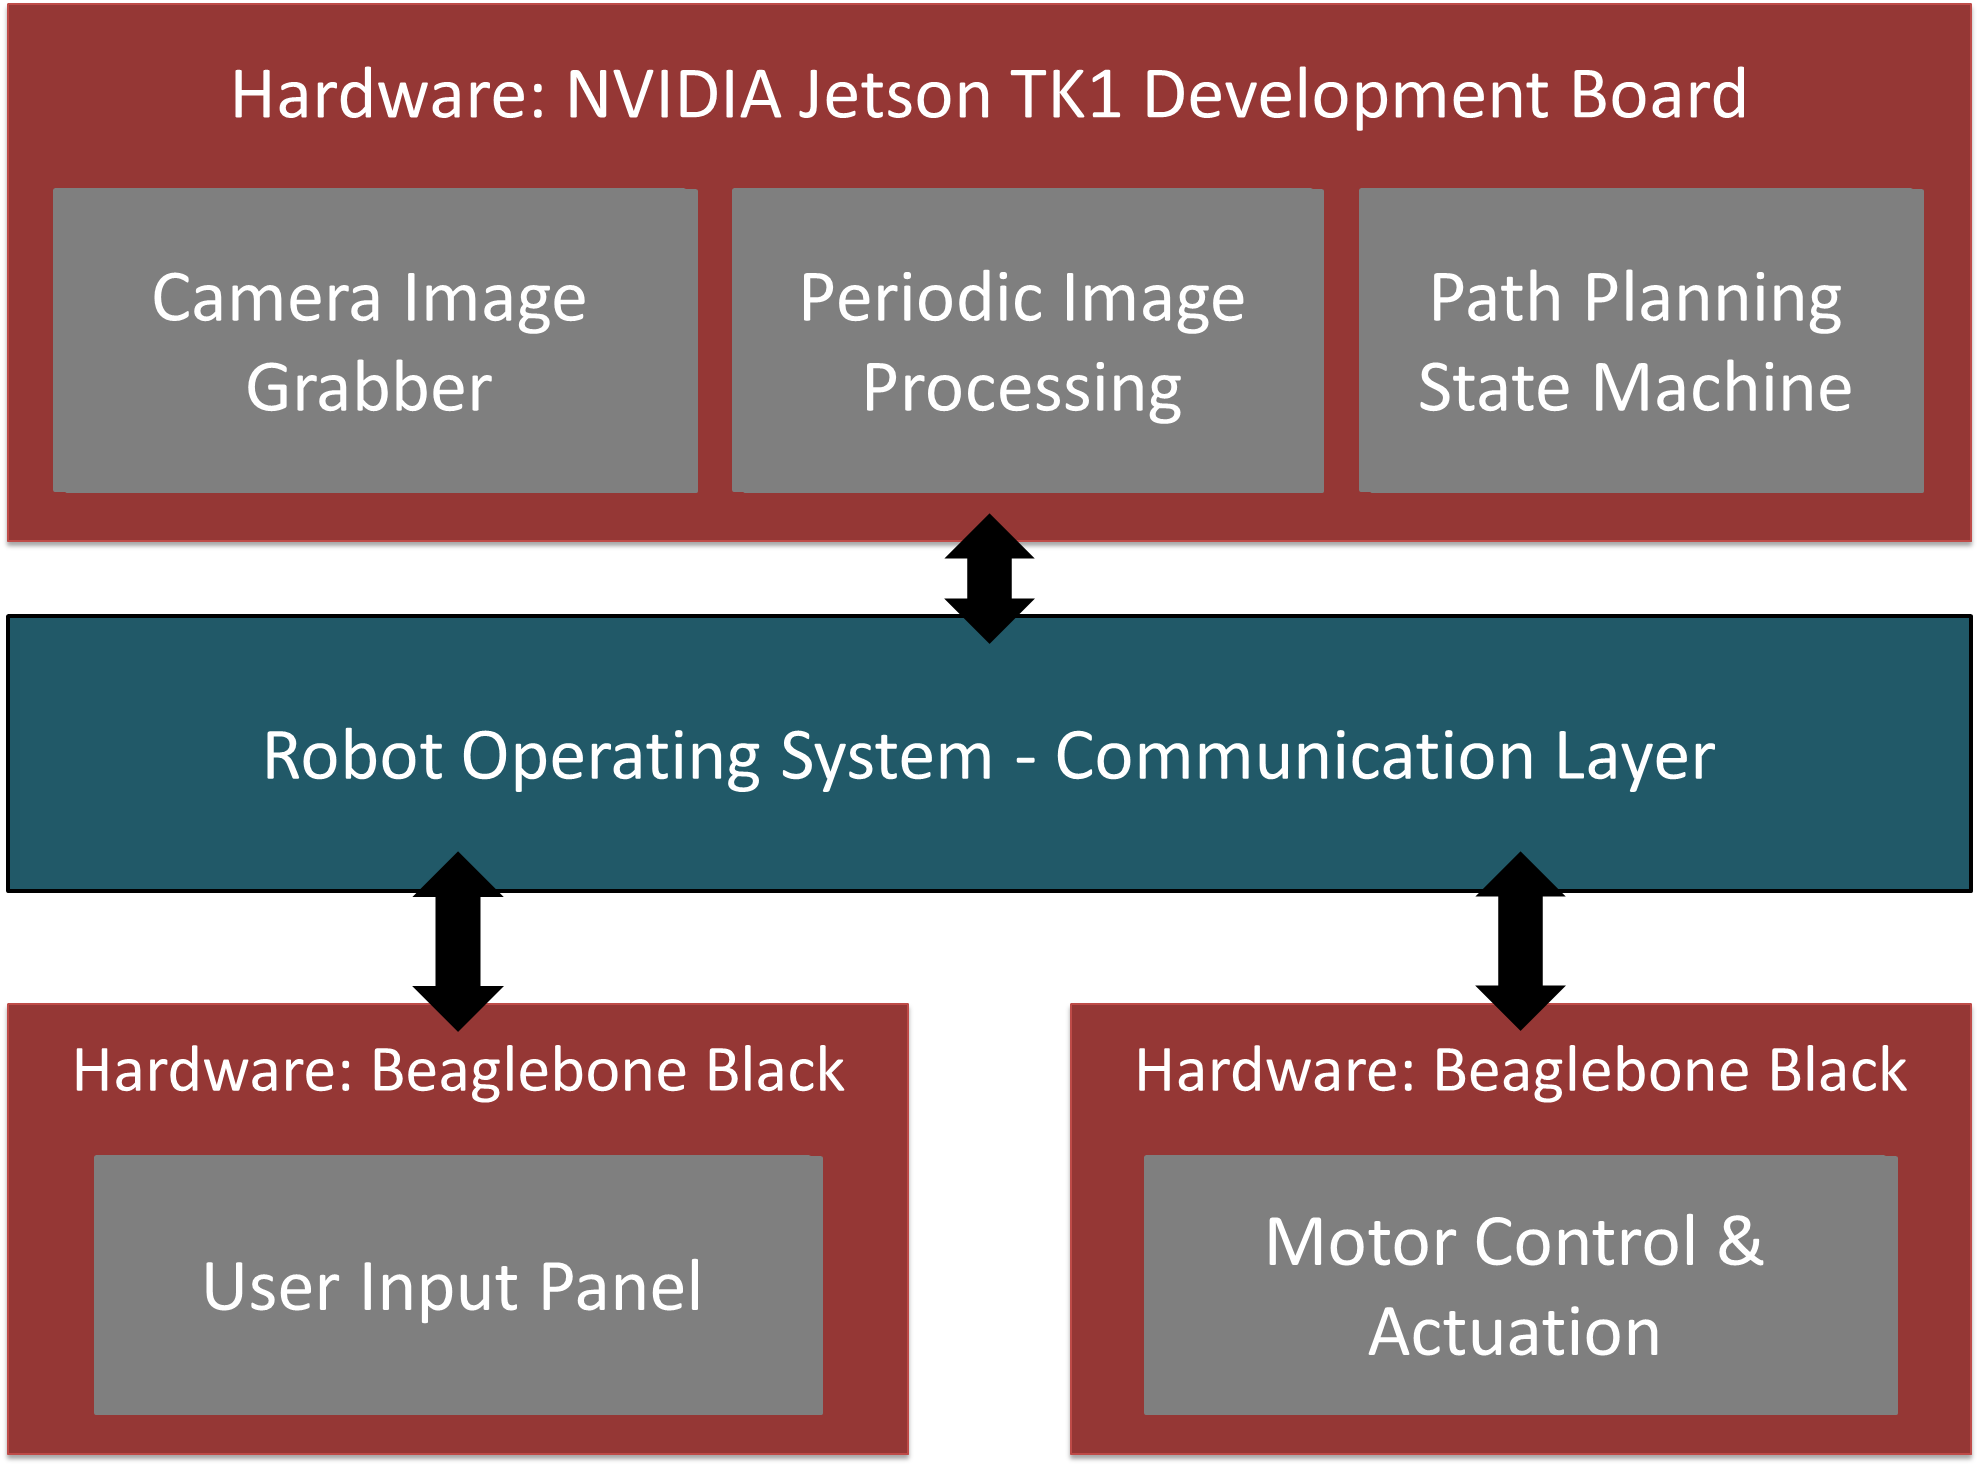
\includegraphics[width=\textwidth]{AGSE_Deployment.png}
	\caption{AGSE Package Deployment}
	\label{fig:AGSE_Deployment}
\end{figure}

The NVIDIA Jetson TK1 periodically fetches the latest webcam feed,
performs image processing and high-level path planning, and updates a
global state machine. The Beaglebone Black (BBB) mounted on top of the
robot performs power management, low-level motor control and feedback
processing. Lastly, the User Input Panel (UIP) houses a second
Beaglebone Black which reacts to user input through switches and
provides feedback through touchscreen display and LED panel
display. The UIP also responsible for keeping the user
informed about the real-time state of the AGSE and the current webcam
feed. Each of these controllers host multiple ROS nodes with ROSMOD
component executor threads periodically performing algorithmic
computations, calculating new robotic paths and communicating to
coordinate and maintain the AGSE state.

\subsubsection{Software Prototyping with ROSMOD}

\begin{figure}[h]
	\centering
	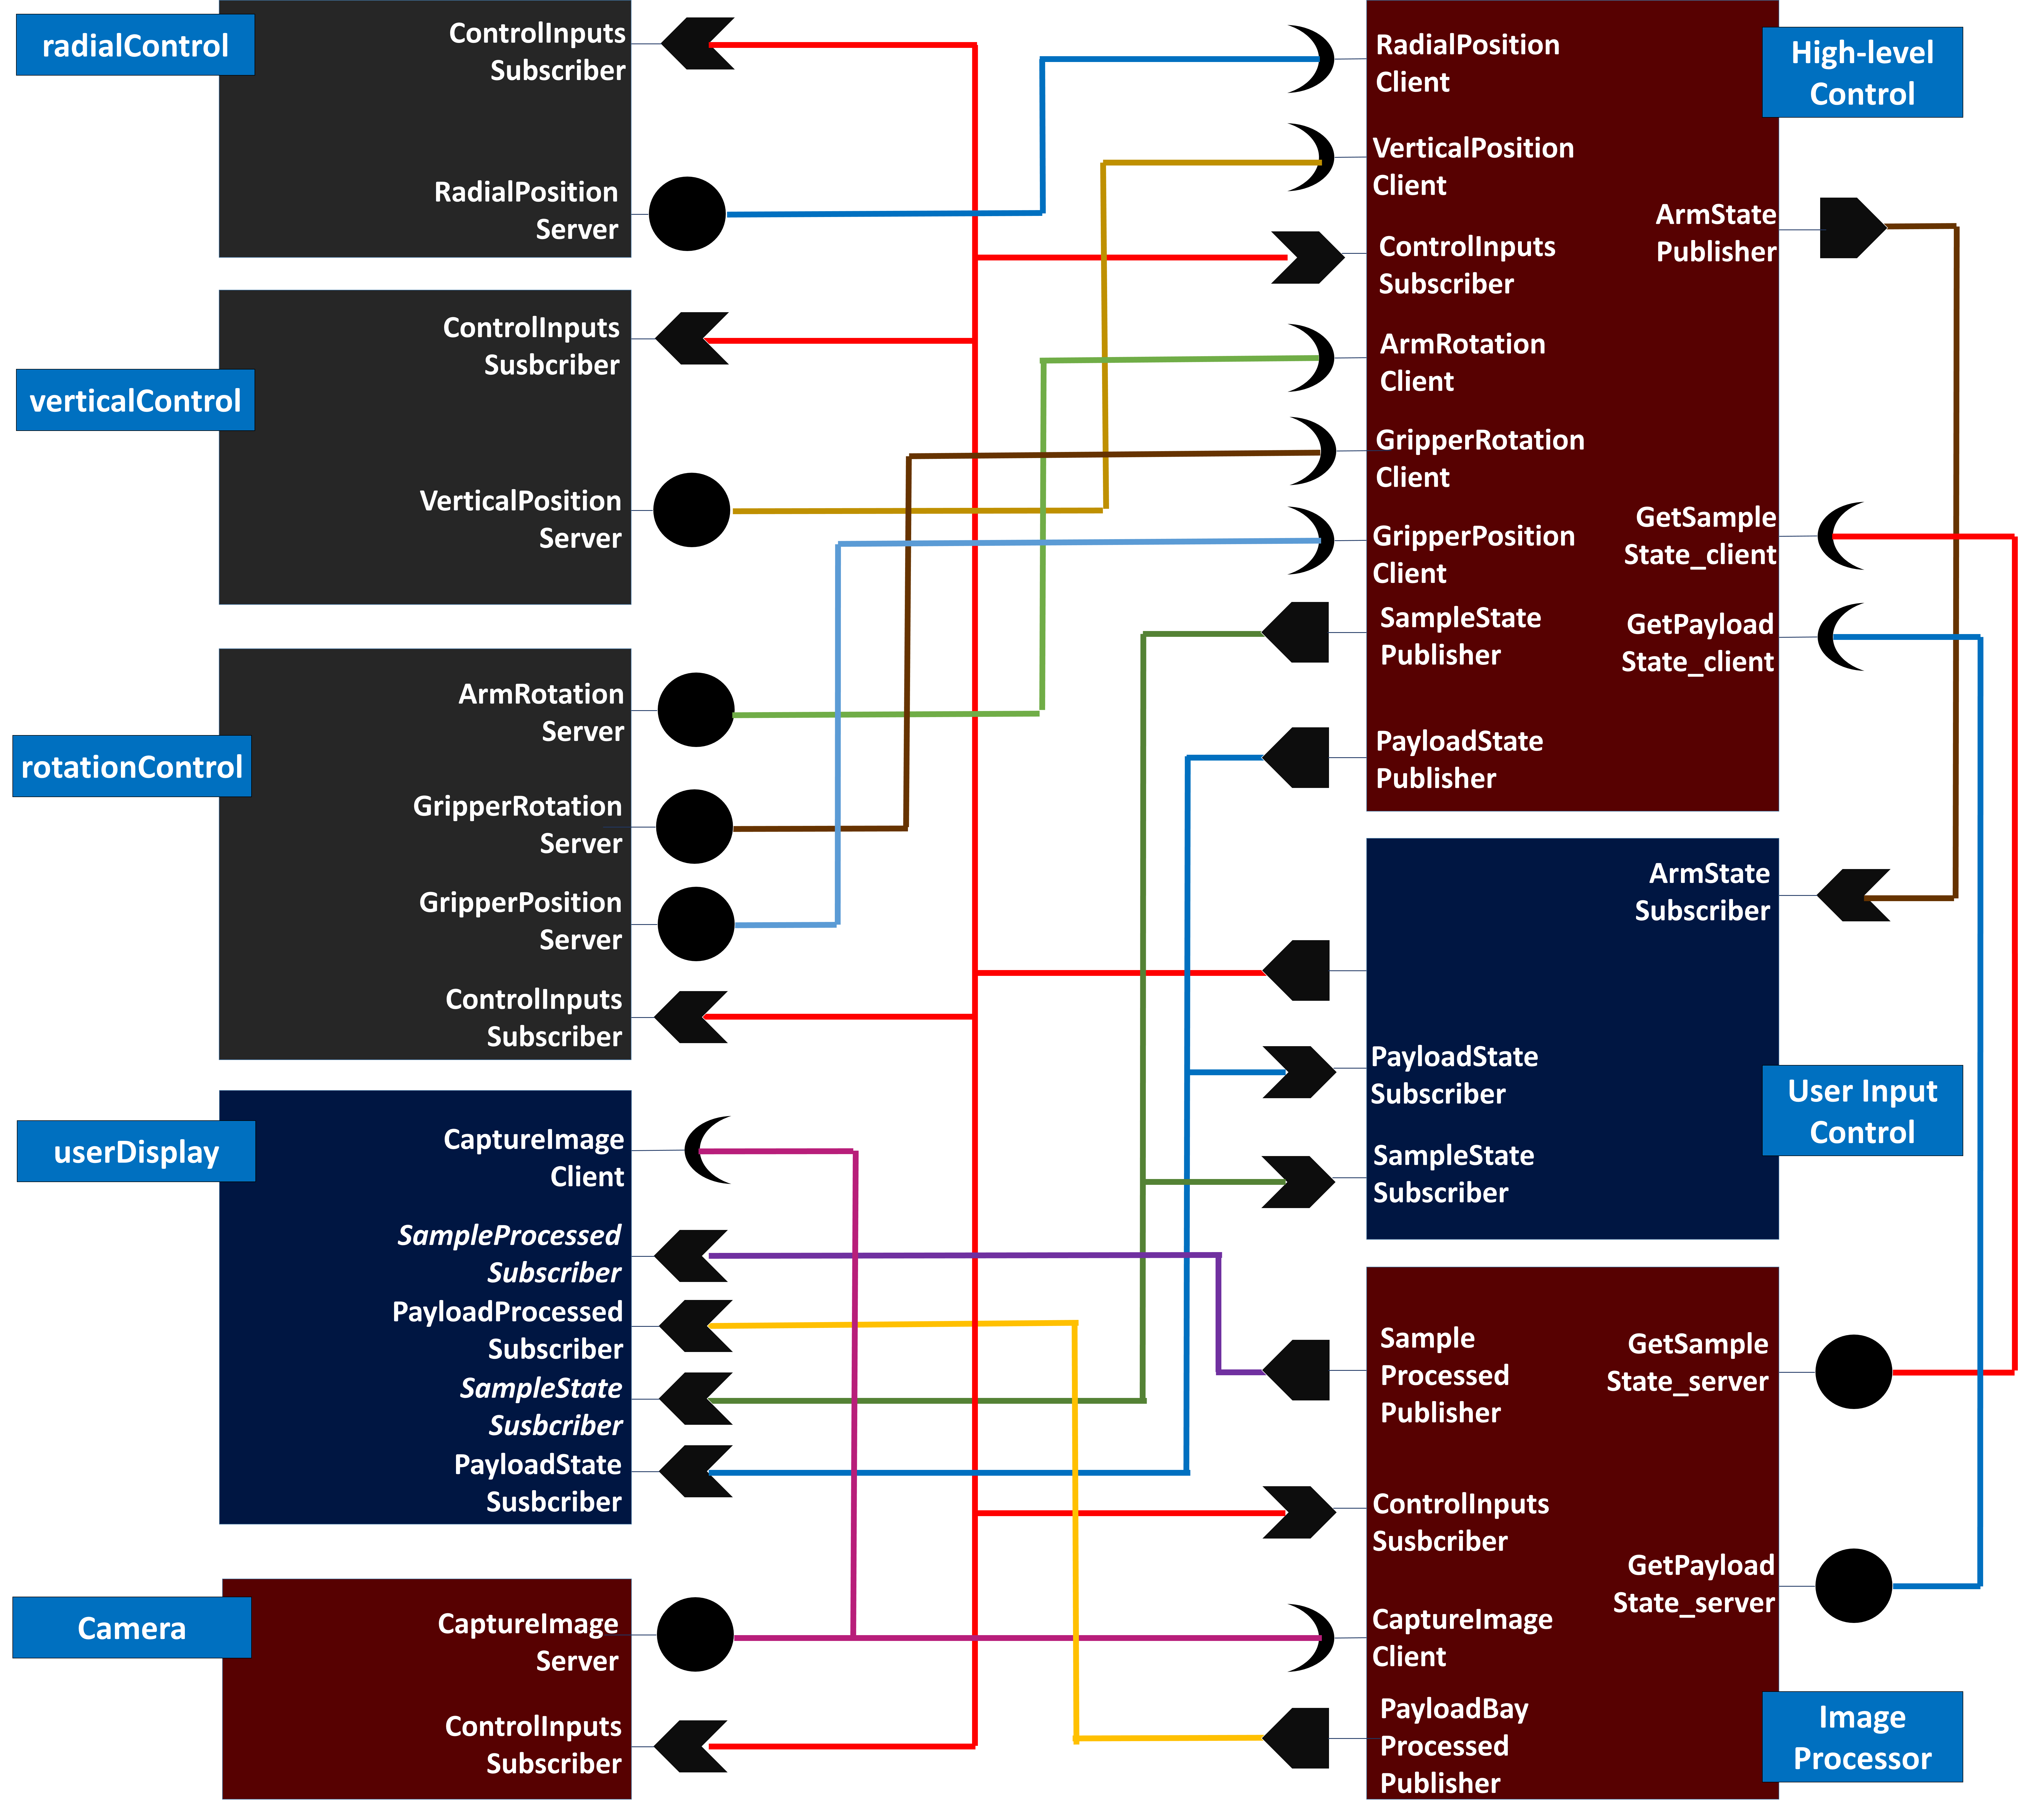
\includegraphics[width=\textwidth]{AGSE-Deployment.png}
	\caption{AGSE Component Assembly}
	\label{fig:AGSE}
\end{figure}

The AGSE software was iteratively designed and rapid prototyped using
our ROSMOD tool suite. The Software Model consists of 8 components
spread across three ROS packages - motor control, high-level state
machine control and image processing. Each package is characterized by
its local set of messages, service and interacting components. Note
that just as in ROS, packages can share messages so that components
can subscribe/publish/provide/require messages/services from other
packages. Figure \ref{fig:AGSE} shows the component assembly and
wiring as per the design. The \emph{radialControl} and
\emph{verticalControl} components are responsible for radial and
vertical actuation of the AGSE respectively. The
\emph{rotationControl} component is capable of controlling three servo
motors: (1) the base rotation servo, (2) the gripper rotation servo,
and finally the (3) gripper position servo that opens and closes the
robot gripper. A \emph{Camera} component deployed on the NVIDIA Jetson
TK1 provides a direct interface to the camera. Using the
\emph{CaptureImage\_Server}, the \emph{ImageProcessor} component
receives a snapshot of the camera feed for periodic processing
needs. This feed is also used by the \emph{userDisplay} component to
display the feed on the user input panel, as shown in Figure
\ref{fig:AGSE_Deployment}. The user input panel is the primary
interface between the ROSMOD applications and the user. The
\emph{userDisplay} component provides information to the user and the
\emph{userInputControl} receives data from the user, specifically to
read the various control switches on the panel e.g. the pause, alarm,
and debug switches. Lastly, a \emph{HighLevelControl} component
orchestrates the high-level state transitions and controls the
operation of the robotic arm. These transitions include commands such
as \emph{find\_payload\_bay}, \emph{find\_sample},
\emph{move\_to\_target} etc., each of which publishes messages to
other components to propagate the motor control commands.

The ROSMOD code generators enabled generation of nearly 60\% (6,000+
lines) of the total built code. As mentioned before, much of this code
includes port initialization, build system files, callback skeletons,
etc. that usually take up a significant amount of development time. As
developers, we had to fill in the missing pieces - the business logic
of the callbacks, completing the component interaction loops. This
code includes architecture-specific control, e.g. GPIO and encoder
readings, LED and switch settings, camera image acquisition, and
high-level control.

The final AGSE used in the 2014-2015 NASA SLI competition is shown in
Figure~\ref{fig:competition_AGSE}.

\begin{figure}[h]
	\centering
	\includegraphics[width=\textwidth]{AGSE_Render.png}
	\caption{AGSE and rocket used in the 2014-2015 NASA SLI
		competition.  The UIP is shown in the bottom left of the
		picture, the Motor Control Board is on the top of the arm of
		the AGSE, and the NVIDIA Jetson is under the rocket.}
	\label{fig:competition_AGSE}
\end{figure}


\subsubsection{Performance Assessment}

At the competition, the Vanderbilt AGSE was able to complete the
sample retrieval process in approximately $4.5$ minutes. The recovery
process, as shown in Figure \ref{fig:AGSE_Operation}, was successful,
with payload and rocket bay recognition occurring quickly and
efficiently. The AGSE was able to grasp the payload using only two of
its four padded end effector phalanges, and successfully deposited the
payload within the rocket bay. This operation received high marks from
the NASA officials and earned the competition's \emph{Autonomous
	Ground Support Equipment Award}.

\begin{figure}[t]
	\centering
	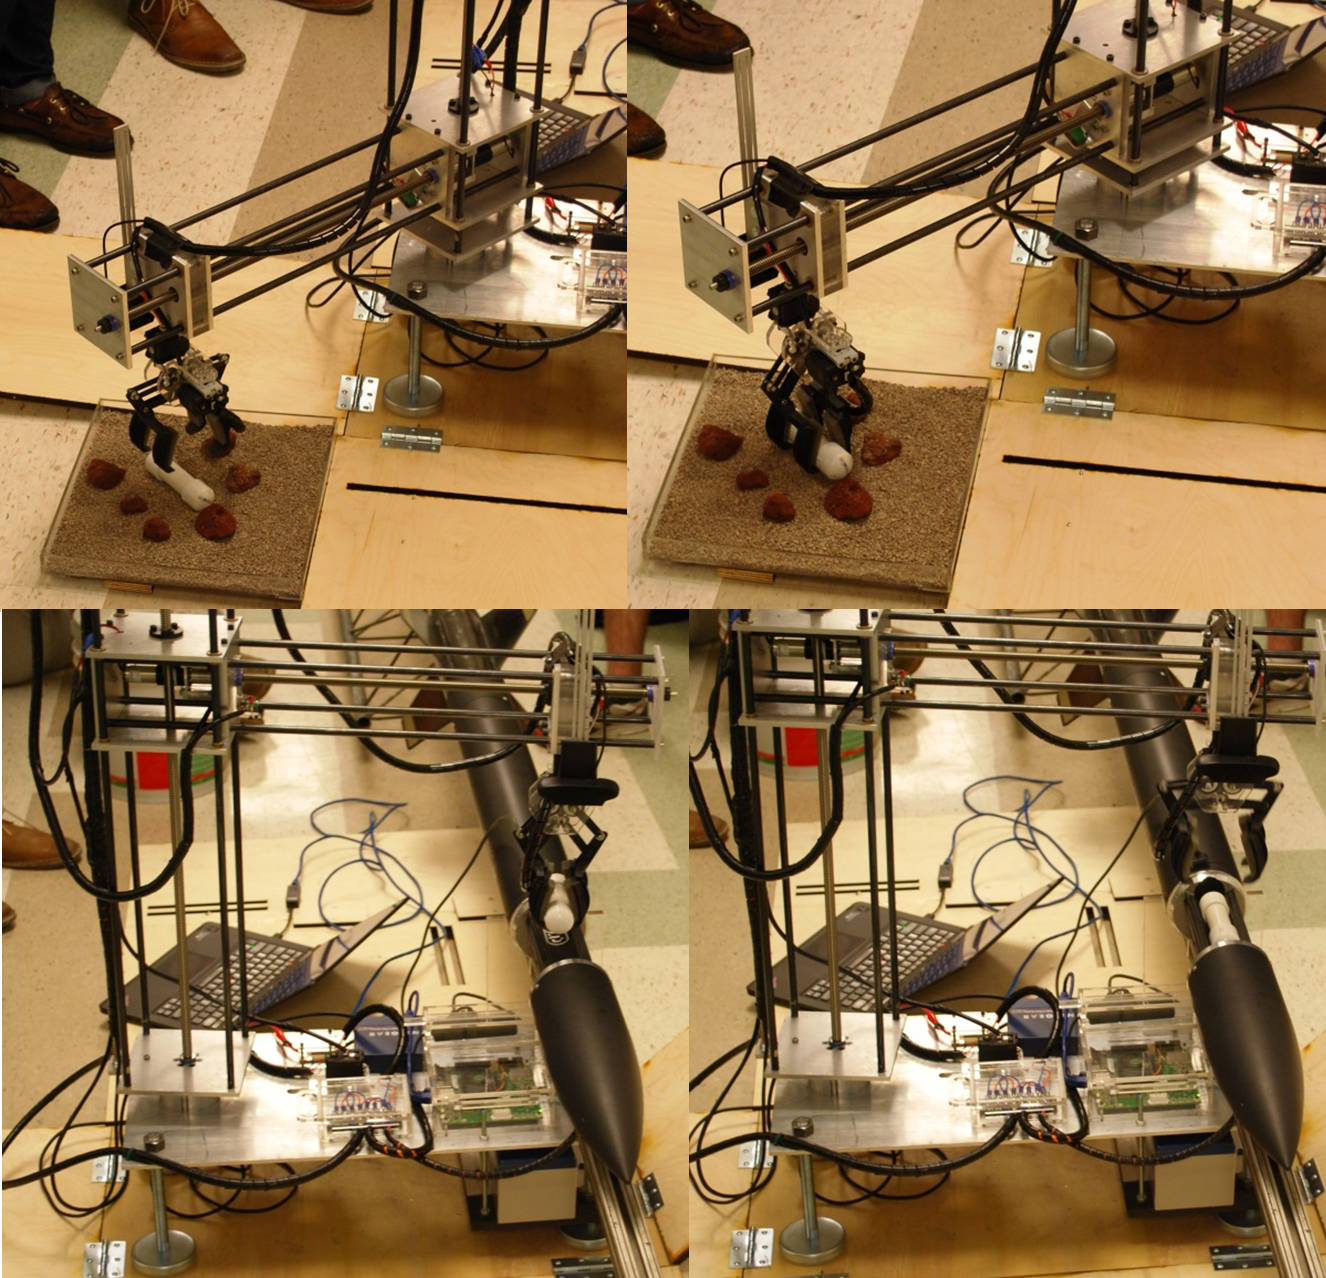
\includegraphics[width=\linewidth]{AGSE_Operation.png}
	\caption{AGSE Calibration and Testing}
	\label{fig:AGSE_Operation}	
\end{figure}

System robustness was validated on the day of competition when a key
component failed and was able to be quickly replaced with a different
part with no detriment to system performance. The Dynamixel AX-12A
servo controlling the base rotational degree of freedom of the AGSE
suffered an irreparable failure of its gearbox and had to be removed
from the robot. A backup of the servo was not readily available, and a
different model servo by the same company had to be swapped in
instead.  This new model, a Dynamixel MX-28T, while having similar
performance as the old servo, had a different communication protocol
and mounting footprint, as well as a more complex control scheme.

The component-based nature of ROSMOD allowed quick modifications of
the business logic of the \emph{rotation\_controller} component to
update the system to use the new hardware.  The new control scheme was
quickly implemented and the control software was updated to account
for the new physical placement of the servo due to its different
mounting footprint. After these modifications were made, the AGSE was
able to perform at its optimal level during its part of the
competition.


